%\documentclass[10pt,twoside,lineno]{GSA_format}
\documentclass[10pt,twoside,lineno, twocolumn]{GSA_format}

% Use the documentclass option 'lineno' to view line numbers
\usepackage[normalem]{ulem}
\usepackage{float}
\usepackage{setspace}
\usepackage{lipsum}
\usepackage{color,soul}


%\doublespacing

\useunder{\uline}{\ul}{}
\articletype{inv} % article type

\newcommand{\bm}[1]{\mbox{\boldmath{$#1$}}}

\newcommand{\beginsupplement}{%
        \setcounter{table}{0}
        \renewcommand{\thetable}{S\arabic{table}}%
        \setcounter{figure}{0}        \renewcommand{\thefigure}{S\arabic{figure}}%
     }

\title{A window-based approach for genotype-environment association studies}

\author[1,2,$\textdollar$]{Tom R. Booker}
\author[3]{Samuel Yeaman}
\author[1,2]{Michael C. Whitlock}
\affil[1]{Department of Zoology, University of British Columbia, Vancouver, Canada}
\affil[2]{Biodiversity Research Centre, University of British Columbia, Vancouver, Canada}
\affil[3]{Department of Biological Sciences, University of Calgary, Calgary, Canada}

\keywords{Local adaptation, population genetics, landscape genomics}

\runningtitle{Incorporating linkage in GEA analyses} % For use in the footer 

\runningauthor{Booker \textit{et al.}}

%Because we use the genome-wide distribution of \textit{p}-values, using 

\begin{abstract}
\textit{I'm using the GENETICS template because it looks nice, but I would like to submit this there}

Genotype environment association (GEA) studies have the potential to elucidate the genetic basis of local adaptation in natural populations. Specifically, GEA approaches look for a correlation between allele frequencies and putatively selective features of the environment. Genetic markers with extreme evidence of correlation with the environment are presumed to be tagging the location of alleles that contribute to local adaptation. In this study, we propose a new method for GEA studies called the weighted-Z analysis (WZA) that combines information from closely linked sites into analysis windows in a way that was inspired by methods for calculating $F_{ST}$. We analyse simulations modelling local adaptation to heterogeneous environments using GEA methods that control for population structure or uncorrected approaches. In the majority of cases we tested, the WZA either performs similarly to single-SNP based approaches or outperforms them. We found that correcting for population structure using an estimated population covariance matrix resulted in a loss of statistical power, similar to results from a previous study. The WZA outperforms individual SNP approaches when the measured environment is not perfectly correlated with the true selection pressure, or the a small number of individuals or demes was sampled.  Finally, we apply the WZA to empirical data from lodgepole pine. \\


\end{abstract}

\begin{document}

\maketitle
%\thispagestyle{firststyle}
\marginmark
\firstpagefootnote


\correspondingauthoraffiliation{$\textdollar$}{Corresponding author: booker@zoology.ubc.ca}
\vspace{-33pt}% Only used for adjusting extra space in the left column of the first page


    %%%%%
      %
      %      
      %
      %
      %
      %
      %
    %%%%%
    
\section{Introduction}

With an understanding of the genes or genomic regions that contribute to local adaptation, we may develop an understanding of the genetic architecture of adaptation and inform models of the limits and constraints of evolvability (e.g. \citealt{Yeaman2018}). In addition, knowledge of the loci or alleles involved in local adaptation may inform conservation management programs for buffering against the consequences of anthropogenic climate change \citep{Aitken2013-yp}.   \\

Alleles may vary in frequency across a species' range in response to changing environmental conditions that give rise to spatially varying selection pressures \citep{Haldane1948}. For that reason, genetic variants that exhibit strong correlations with putatively selective features of the environment are often interpreted as a signature of local adaptation \citep{Coop2010}. Genotype-environment association (GEA) studies examine such correlations. Allele frequencies for many genetic markers, typically single nucleotide polymorphisms (hereafter SNPs), are estimated in numerous locations across a species's range. Correlations between allele frequency and environmental variables are calculated then contrasted for sites across the genome. It is assumed in GEA studies that current heterogeneity in the environment (whether biotic or abiotic) reflects the history of selection. \\
%In the context of GEA studies, the term environment may refer to any abiotic or biotic variable that the species of interest could conceivably be adapting or have adapted to. \\

%% Add something about GWAS approaches
Numerous approaches for performing GEA analyses have been proposed. If individuals are sequenced, GEA can be performed by regressing environments on genotypes as a form of genome-wide association study, for example using the \textit{GEMMA} package \citep{Zhou2013}. However, to estimate SNP effects with reasonable statistical power, many individuals may need to be sequenced. A cost-effective alternative is pooled sequencing (hereafter pooled-seq), where allele frequencies for populations of individuals are estimated rather than individual genotypes \citep{Schlotterer2014}. In this study, we focus on analyses that can be performed on pooled-seq datasets given the wide adoption of that protocol in the GEA literature.\\

The most straightforward way to perform a GEA analysis is to simply examine the correlation between allele frequencies and environmental variables measured in multiple populations, for example using rank correlations such as Spearman's $\rho$ or Kendall's $\tau$. This simple approach may commonly lead to false positives, however, if there is environmental variation across the focal species's range that is correlated with patterns of gene flow or historical selection \citep{Meirmans2012,Novembre2009}. For example, consider a hypothetical species inhabiting a large latitudinal range. If the hypothetical species had restricted migration and exhibited isolation-by-distance, neutral alleles may be correlated with any environmental variable that happened to correlate with latitude simply due to population structure.  \\

%In the case of pool-seq , the input to GEA is a $j \times n$ allele frequency matrix, where $j$ is the number of populations sampled and $n$ is the total number of SNPs. Alternatively, researchers may sequence individuals from particular environments. In the case of individual-seq, the input to GEA is a $x \times n$ genotype matrix, where $x$ is the number of individuals sequenced. 

Several approaches have been proposed to identify genotype-environment correlations above and beyond what is expected given underlying population structure. The commonly used BayPass \citep{Gautier2015} package, which is an extension of BayEnv by \cite{Coop2010}, estimates correlations between alleles and environmental variables in a two-step process. First, a population covariance matrix (\textbf{$\mathbf{\Omega}$}) is estimated from SNP data. Second, correlations between the frequencies of individual SNPs and environmental variation is estimated treating \textbf{$\mathbf{\Omega}$} in a manner similar to a random effect in a generalised mixed model. Latent-factor mixed models (LFMM) are an alternative approach for performing GEA \citep{Frichot2013}, and are implemented in the LEA package \citep{Frichot2015}. In LFMMs, an allele frequency matrix is regressed on environments with population structure modelled as a series of 'latent factors', which are major axes of variation in the allele frequency matrix. For clarification, if one ran an LFMM on SNP data without environmental data and set the number of latent factors equal to the number of loci in the allele frequency matrix, the result would be similar to calculating the loadings in a principle components analysis. Finally, redundancy analysis (RDA) has been proposed as a way to perform GEA studies incorporating multiple environmental variables \citep{Forester2016, Forester2018}. In RDA, a multiple regression of allele frequencies at each SNP on environmental variables is performed. This leads to a matrix of fitted values with the same dimensions as the allele frequency matrix. A principle components analysis is then performed on the matrix of fitted values and the loadings on the first few axes of variation are used as test statistics \citep{Legendre2012}. Note that RDA does not explicitly control for population structure. A recent study used simulated data to compare the performance of the GEA methods we have outlined \citep{Lotterhos2019-ki}. Overall, \cite{Lotterhos2019-ki} found that a comparatively simple analysis calculating Spearman's $\rho$ between allele frequency and environment performed similarly to RDA, as measured by precision-recall curves, and both uncorrected approaches outperformed LFMMs and \textit{BayPass}. In all of the GEA analysis methods outlined above, each SNP is treated independently, though the "AUX" mode in \textit{BayPass} can account for linkage disequilibrium by modelling the spatial dependency among SNPs. However, the "AUX" mode is recommended for zeroing in on particular regions rather than genome-wide scans \citep{Gautier2015}.\\

Closely linked SNPs are not independently inherited and may have highly correlated evolutionary histories. Individual SNPs may provide very noisy estimates of summary statistics, but by combining information across closely linked sites noise can be reduced. It is for that reason that genome scan studies often aggregate data across adjacent markers into analysis windows based on a fixed physical or genetic distance or number of SNPs \citep{Hoban2016}. In the case of $F_{ST}$, the standard measure of population differentiation, there are numerous methods for combining estimates across sites (\textit{See} \citealt{Bhatia2013}). In Weir and Cockerham's (\citeyear{Weir1984-tc}) method, for example, estimates of $F_{ST}$ for individual loci are combined into a single value with each marker's contribution weighted by its allele frequency. \\

In the context of GEA studies, each marker or SNP provides a test of whether a particular genealogy is correlated with environmental heterogeneity. In the extreme case of a non-recombining region, each SNP would be present on the exact same genealogy and thus provide a test of identical hypotheses. However, the SNPs that are the most informative in this context are those at high frequencies as they contain the most information about the shape of the underlying genealogy. For recombining portions of the genome, however, linked sites will not have the exact same genealogy, but genealogies may be highly correlated. Similar to combining estimates of $F_{ST}$ to decrease statistical noise, combining GEA tests performed on individual markers into analysis windows may increase the power of GEA studies to identify genomic regions that contribute to local adaptation. \\

In this study, we propose a general method for combining the results of single SNP GEA scores into analysis windows that we call the weighted-Z analysis (WZA). Using simulations, we generate datasets modelling a pooled-sequencing experiment where estimates of allele frequency are obtained for numerous populations across a species' range. We analyse our simulated data and compare the performance of the WZA to current GEA approaches. We show that the WZA is particularly useful when GEA analyses on individual SNPs are noisy. We re-analyse previously published lodgepole pine data using the WZA and find several candidate loci that were not identified using the methods of the original study. 


%%     %%
% %   % %
%  % %  %
%   %   %
%       % 
%       %
%       %
%       %
%       %
%       %

\subsection{\underline{The Weighted-Z Analysis}} 

In this study, we propose the Weighted-Z Analysis (hereafter, the WZA) for combining information across linked sites in the context of GEA studies. The WZA uses the weighted-Z test, a test from the meta-analysis literature that combines \textit{p}-values from multiple independent hypothesis tests into a single score. In the weighted-Z test, each of the $n$ independent tests is given a weight that is proportional to the inverse of its error variance \citep{WHITLOCK2005}. Inspired by Weir and Cockerham's (\citeyear{Weir1984-tc}) method for combining estimates of $F_{ST}$ across sites, in the WZA we use a marker's allele frequency to determine weights when performing the weighted-Z test on GEA data. At a given polymorphic site, we denote the average frequency of the minor allele across populations as $\overline{p}$ ($\overline{q}$ corresponds to the major allele). The sampling variance of frequency for the minor allele from one generation to the next is $\frac{\overline{p}\overline{q}}{2N}$, where $N$ is the population size \citep{RN173}.  In the WZA, we $\overline{p}\overline{q}$ in place of the error variance in the weighted-Z test. \\

We combine information from the markers (typically SNPs) present in a focal genomic region into a single weighted-Z score ($Z_W$). The genomic region in question could be a gene or genomic analysis window. We calculate $Z_{W,k}$ for genomic region \textit{k}, which contains \textit{n} SNPs as

\begin{equation}
\label{weightedZ}
Z_{W,k} =  \frac {\sum\limits_{i=1}^n \overline{p_i} \overline{q_i}z_i}{\sqrt{ \sum\limits_{i=1}^n (\overline{p_i}\overline{q_i})^2} },
\end{equation}

\noindent where $z_i$ is the standard normal deviate calculated from the one-sided \textit{p}-value for SNP \textit{i}. \\

A feature of the WZA is that many statistics can potentially be used as input as long as individual SNPs provide a measure for the strength of evidence against a null hypothesis. \\

Under the null hypothesis that there is no correlation between allele frequency and environment, the expected distribution of correlation coefficients in a GEA would be normal about 0, with a uniform distribution of \textit{p}-values. However, as will often be the case in nature, there may be an underlying correlation between population structure and environmental heterogeneity that will cause these genome-wide distributions to deviate from this null expectation. The average effect of population structure on individual SNP scores can be incorporated into an analysis by converting an individual SNP's correlation coefficient or parametric \textit{p}-value into empirical \textit{p}-values based on the genome-wide distribution. With this procedure, we lose some ability to ascribe significance to particular regions, but aggregating the empirical \textit{p}-values using the WZA may identify genomic regions with a pattern of GEA statistics that deviate from the average genome-wide. In empirical studies, it may be preferable to use the parametric \textit{p}-values rather than the correlation coefficients themselves as there may be varying power to calculate correlations across the genome, e.g. due to varying levels of missing data. \\

When we apply the WZA in this study, we used two different statistics as input. The first was empirical \textit{p}-values calculated from the genome-wide distribution of parametric \textit{p}-values from Kendall's $\tau$. The second is empirical \textit{p}-values calculated from the genome-wide distribution of Bayes factors as obtained using the \textit{BayPass} program (see below). 

%Hancock et al (2011), incorporated the average effect of population structure into their GEA analysis of European \textit{Arabidopsis} by converting the distribution of parametric \textit{p}-values for the correlation of individual SNPs and the environment into empirical \textit{p}-values. 

\section{Materials and Methods}
\label{sec:materials:methods}


\subsection{\underline{Simulating local adaptation}} 

We performed forward-in-time population genetic simulations of local adaptation to test the WZA and compare its performance to the commonly used \textit{BayPass} package. GEA studies are often performed on large spatially extended populations that may be comprised of hundreds of thousands of individuals. However, it is computationally infeasible to model selection and linkage in long chromosomal segments (>1Mbp) for such large populations. For that reason, we simulated relatively small populations containing 19,600 diploid individuals in total and scaled population genetic parameters so as to model a large population. We based our choice of population genetic parameters on estimates for conifer species and in the Appendix we give a breakdown and justification of the parameters we simulated. A representative set of parameters is given in Table \ref{tab:SimulationParameters}. All simulations were performed in SLiM v3.4 \cite{Haller2019}. \\

The simulated organism had a genome containing 1,000 genes uniformly distributed onto 5 chromosomes. We simulated a chromossome structure in SLiM by including nucleotides that recombined at \textit{r} = 0.5 at the hypothetical chromosome boundaries. Each chromosome contained 200 10,000bp long segments. We refer to these segments as genes for brevity, although we did not model an explicit exon/intron or codon structure. Recombination within genes was uniform and occurred at a rate of $r = 10^{-7}$, giving a population-scaled recombination rate ($4N_dr$) of 0.0004. The final base-pair in each gene recombined at a rate of 0.005, effectively modelling a stretch of 50,000bp of intergenic sequence. \\

Individuals inhabited a 2-dimensional stepping-stone population made up of 196 demes (i.e. a $14\times14$ grid). Each deme consisted of $N_d$ = 100 diploid individuals. We assumed a Wright-Fisher model so demes did not fluctuate in size over time. Migration was limited to neighbouring demes in the cardinal directions and the migration rate ($m$) was set to $m = \frac{7.5}{2N_d}$ in each possible direction to achieve an overall $F_{ST}$ for the metapopulation of around 0.04 (Figure \ref{fig:summaryStats}). Additionally, we simulated metapopulations with no spatial structure (i.e. finite deme island models). In these simulations, we used formula $m = \frac{\frac{1}{F_ST} - 1}{4N_d196}$ (\citeauthor{RN173} \citeyear{RN173} pp319) to achieve a target $F_{ST}$ of 0.03.\\

In nature, species may inhabit large spatial ranges and environmental variation may shape selection pressures. Obviously environmental variation is autocorrelated in space, so when modelling local adaptation to variable environments incorporating realistic spatial autocorrelation may be important. \\

We incorporated spatial heterogeneity in the environment into our simulations using a discretised map of degree days below 0 (DD0) across British Columbia (BC). We generated the discretised DD0 map as follows. We downloaded the map of DD0 for BC from ClimateBC (http://climatebc.ca/; \cite{Wang2016}). From the DD0 map (Figure 1A). Using Dog Mountain, BC as the reference point in the South-West corner (Latitude = 48.37, Longitude = -122.97), we extracted data in a rectangular grid with edges 3.6 degrees long in terms of both latitude and longitude, an area of approximately $266\times400 km^2$ (Figure 1A). We divided this map into a $14\times14$ grid, calculated the the mean DD0 scores in each grid cell, converted them into standard normal deviates (i.e. Z-scores) and rounded up to the nearest third. We used the number of thirds of a Z-score as phenotypic optima in our simulations. We refer to this map of phenotypic optima as the \textit{BC} map.\\

We used data from the \textit{BC} map to generate two additional maps of environmental heterogeneity. First, we ordered the data from the \textit{BC} map along one axis of the $14\times14$ grid and randomised optima along the non-ordered axis. We refer to this re-ordered map as the \textit{Gradient} map (Figure 1C). Both the BC map and the gradient map have a normally distributed range of phenotypic optima. For some species, selection may only apply beyond a certain environmental threshold, leading to a non-normal distribution of phenotypic optima. To model such a situation, we set the phenotypic optimum of 20 demes in the top-right corner of the meta-population to +3 and set the optimum for all other populations to -1. We chose 20 demes as it represented 10.2\% of the total population. We refer to this map as the \textit{Truncated} map (Figure 1D).\\

%We simulated environmental variables that were correlated with the phenotypic optimum using Cholesky decomposition of the correlation matrix.


%We constructed a map using data for real climate variation from British Columbia, Canada. We downloaded the map of degree days greater than 0 for British Columbia from ClimateBC (website; REF). From the DD0 map, we extracted the data for a 99x99 grid using Dog Mountain, BC as the reference point in the South-West corner. We divided this map into a 16x16 grid and calculated the mean DD0 for each cell. We converted the means into Z-scores and rounded values up to the nearest third of a Z-score. These data were then used as the phenotypic optima for a structured population models in SLiM.

We used either directional or stabilising selection to model local adaptation. In both cases, there were 12 genes distributed evenly across four of simulated chromosomes that potentially contributed to local adaptation. When assuming directional selection, fitness affecting mutations could only occur at a single nucleotide position in the centre of the 12 potentially selected genes. Directionally selected mutations had a spatially antagonistic effect on fitness. In deme \textit{d} with phenotypic optimum $\theta_d$, the fitness of a selected allele was calculated as $1 + s_a\theta_d$ for an individual homozygous for a locally beneficial allele. The directional selection simulations had a mutation rate of $10^{-7}$.  \\

When assuming stabilising selection, the phenotypic effects of mutations that occurred in the 12 genes had a normal distribution of phenotypic effects, with variance $\sigma_a^2 = 0.5$. Phenotype affecting mutations occurred at a rate of $10^{-10}$ per base-pair in the 12 genes. An individual's phenotype was calculated as the the sum of the phenotypic effects of all phenotype affecting mutations. We calculated an individual's fitness using the standard expression for Gaussian stabilising selection,
\begin{equation}
\notag
W[z_{i,j} = exp \Big[\frac{-(f_{i,j} - \theta_d)^2}{2V_s}\Big],
\end{equation}
where $f_i$ is the phenotype of the $i^{th}$ individual in environment $j$ and $V_s$ is the variance of the Gaussian fitness function \citep{Walsh}. We set $V_s = 196$ so that there was a 50\% fitness difference between individuals perfectly adapted to the  two extremes of the distribution of phenotypic optima. This was motivated by empirical studies of local adaptation that have demonstrated such fitness differences in numerous species \citep{Hereford2009, Bontrager2020}.\\ 

We ran simulations for a total of 200,102 generations. The 19,600 individuals initially inhabited a panmictic population that evolved neutrally. After 100 generations, the panmictic population divided into the $14\times14$ grid and evolved strictly neutrally when modelling directional selection), or with a phenotypic optimum of 0 for all demes (when modelling stabilising selection). After 180,000 generations, we imposed the various maps of phenotypic optima and simulated for further 20,000 generations.  For selected mutations, we used the "\textit{f}" option for SLiM's mutation stack policy, so only the first mutational change was retained. Using the tree-sequence option in SLiM \citep{Haller2019-za} we tracked the coalescent history of each individual in the population. At the end of each simulations, neutral mutations were added at a rate of $10^{-8}$ usipysling PySLiM (\url{https://pyslim.readthedocs.io/en/latest/}). For each combination of map and mode of selection, we performed 20 replicate simulations. \\


\begin{figure*}
  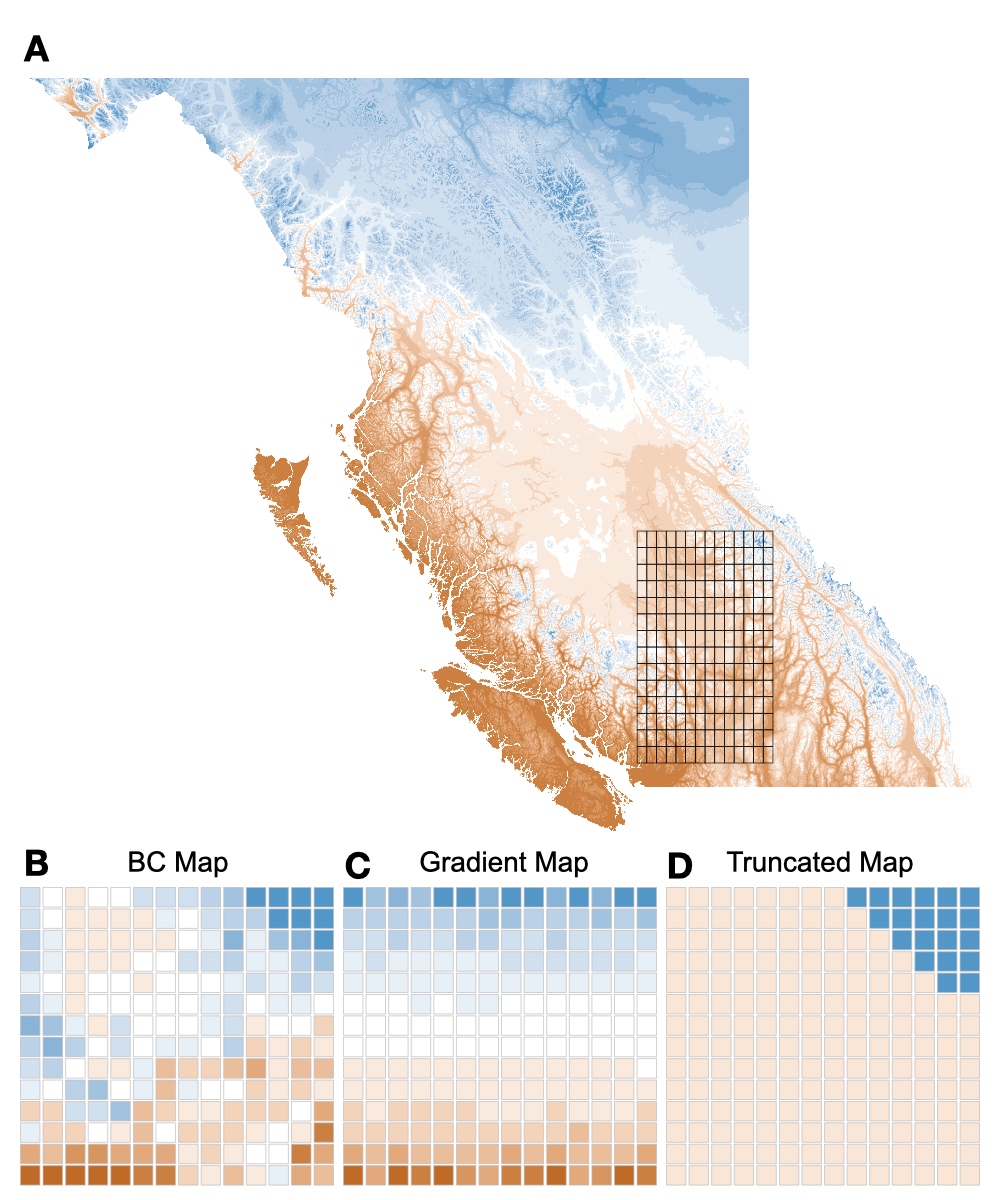
\includegraphics[width=0.5\linewidth,keepaspectratio]{Plots/Figure1/Figure1}
  \caption{A) Degree days below zero across British Columbia, the overlain grid in A shows the locations we used to construct phenotypes for our simulated populations. B) A discretized map of DD0 in Southern British Columbia, we refer to the map in B as the BC map. C) A 1-dimensional gradient in phenotypic optimum, we refer to this as the 1D gradient map. D) A heterogenous distribution of phenotyic optima.}
  
  \label{fig:envGridPlot}
\end{figure*}


\subsection{Classifying genes as locally adapted} 

To evaluate the performance of different GEA methods, we needed to know which genes contribute to local adaptation and which do not in our simulated data. As described above, our simulations incorporated a stochastic mutation model so from replicate to replicate the genes that contributed to local adaptation varied and, in the case of stabilising selection, so did the effect size of the alleles in those genes. The condition we set to determine whether a gene was involved in local adaptation was by measuring the covariance of fitness contributed by alleles present in a particular gene in a particular environment and environmental heterogeneity. For a genetic variant to be considered locally adaptive, there needs to be a positive covariance between the fitness advantage it confers and phenotypic optima across space. \\

We calculated the covariance between environmental heterogeneity and the fitness or phenotypic contribution of a gene for directional and stabilising selection simulations, respectively. For each gene that could potentially contribute to local adaptation there are $k$ causal SNPs. In deme $d$, there are $n$ diploid individuals so we have $\bm{M_{g,d}}$, an $n \times k$ matrix in which the genotype of each individual in $d$ at each causal SNP is coded as 0, 1 or 2 corresponding to aa, aA and AA genotypes, respectively. Under directional selection, each gene that could contribute to phenotypic variation had at most a single causal SNP ($k = 1$) with a selective effect of $\theta_ds_a$. For each gene we calculated the covariance between $\bm{M_{g,d}}\theta_ds_a$ and environmental heterogeneity. Under stabilising selection, we calculated the proportion of covariance between the phenotypic contribution of a gene in a particular deme and the environment. We use $\bm{\nu_g}$ to refer to the vector of phenotypic effects for each of the $k$ causal SNPs in gene $g$. The mean contribution that a gene makes to the phenotype in a particular deme is calculated as $P_{g,d} = \frac{1}{k}\sum \bm{M_{g,d} \nu_{g,d}}$. We took the covariance between $PB_{g,d}$ and the vector of phenotypic optima as our measure of local adaptation for stabilising selection simulations. 

% The variance in $C_{g,d}$ gives us a measure of the phenotypic variance between popuatlions generated by each gene ($\sigma^{2}_{PB,g}$). We then calculate the proportion of variance explained by each gene ($PVE_g$) as $\sigma^{2}_{PB,g} / \sigma^{2}_{PB}$
%\begin{equation}
%PVE_g = \frac{\sigma^{2}_{PB,g}}{\sigma^{2}_{PB}}.
%\end{equation}

%Note that $PVE_g$ does not provide a measure of local adaptation, merely a measure of how much phenotypic variation between populations can be explained by a a particular gene. 

%We recorded the Cov(fitness, environment) as a measure of a gene's relevance to local adaptation in a particular simulation replicate. The three upstream and three downstream genes.

%In our simulations, we used the covariance between the average effect size of a gene in a population and the environment as a measure of a gene's relevance for local adaptation. We calculated the average effect size of a gene as follows.

%We then used Cov($PB_g$, $env$)/Cov($PB$, $env$) as a measure of a gene's contribution to local adaptation.


%We added neutral mutations to each simulated tree sequence at a rate of $1\times10^{-8}$. While this gave us a population scaled mutation rate of $4N_ed\mu = 0.00078$, and resulted in an average of 30 SNPs per gene that passed a minor allele frequency filter of 0.05.
\subsection{Analysis of simulation data}

We performed GEA on our simulated data using either Kendall's $\tau$, a rank correlation that does not model population structure, or \textit{BayPass}, a commonly used package for estimating correlations between allele frequencies and environments while correcting for a population covariance matrix \citep{Gautier2015}. For all analyses, except where specified, we analysed data for set of 40 randomly selected demes and sampled 50 individuals from each to estimate allele frequencies. We sampled individuals from the same set of 40 demes for all analyses (Figure \ref{fig:sampleMaps}). From a given replicate, we calculated Kendall's $\tau$ between population-specific allele frequencies and the local environment for each SNP. Any SNP with an average minor allele frequency less than 0.05 across demes was filtered out. We ran \textit{BayPass} (v2.1; \citealt{Gautier2015}) on simulated data following the "worked example" in section 5.1.2 of the manual provided with the software. 

For each gene in a given simulation replicate, we applied the WZA to either the \textit{p}-values from Kendall's $\tau$, converted into empirical \textit{p}-values or Bayes factors from \textit{BayPass}, converted into empirical \textit{p}-values. 

We used three different methods to summarise the GEA results for each gene, the WZA, the top-candidate method developed by \cite{Yeaman2016} and a single SNP-based approach.

\cite{Yeaman2016} proposed the top-candidate method for combining information across sites in GEA studies that they referred to as the top-candidate method. The top-candidate method attempts to identify regions of the genome involved in local adaptation under the assumption that such regions may contain multiple sites that exhibit strong correlation with environmental variables. The top-candidate method asks whether there is a significant excess of "outlier" SNPs in a region compared to what one would expect given the genome wide distribution. To apply the top-candidate method \cite{Yeaman2016} classified \textit{p}-values below the 1st percentile genome-wide as outliers. The number of outliers in a given genomic region is tested against the average number of outliers seen in a gene. A binomial test is then used to determine whether a given gene has an excess of outliers relative to the genome-wide expectation. Analysis windows or genes with a \textit{p}-value from the binomial test less than 0.0001 were taken as "top-candidates" for local adaptation. In this study, we do not use the \textit{p}-value from the binomial test to categorise windows as being significant or not, we use it as a continuous index.


\subsection{Single SNP-based approach} 

We used a single SNP-based approach to identify genes as outliers in the analysis of GEA data. For each gene, the SNPs with the most extreme test statistic (i.e. smallest \textit{p}-value or largest Bayes factor) for each gene were recorded. 

 was recorded, when using the uncorrected approach or \textit{BayPass}, respectively, all other SNPs were ignored. The most extreme 

Across a simulated genome, the gene containing the SNP with the most extreme test statistic (e.g. the smallest \textit{p}-value) was scored as a hit and other SNPs in the identified gene were subsequently ignored. The gene with the second-most extreme test statistic was then examined, then the third, and so on. 


To assess the performance of the different tests, we examined the genes with the most extreme test statistics and asked whether they contributed to local adaptation. We examined the top 1, 2, 3,... 50 genes in terms of $Z_W$ scores, $-log[10](p$-values) from the top-candidate method, or the SNP-based approach scores. For simulations modelling directional selection, we assessed statistical power by examining the total number of genes that contribute to local adaptation among the test set. Genes that had had a Cov($PB_g$, $env$) > 0.005 were classified as true positives. For the stabilising selection simulations we calculated the proportion of Cov($PB$, $env$) explained by a given set of genes. We calculated the false discovery rate using the total number of genes with that do not contribute to local adaptation in a given set of genes. \\

We examined the properties of the WZA in regions of low recombination by manipulating the tree-sequences we recorded in \textit{SLiM}. In our simulations, genes were 9,999bp long, so to model genomic regions of low recombination rate, we extracted the coalescent trees that corresponded to the central 1,000bp or 100bp of each gene. For the 1,000bp and 100bp intervals, we added mutations at 10$\times$ and 100$\times$ the standard mutation rate. \\

Tree sequences were manipulated using the tskit package. Mutations were added to trees using msprime (REF) through the PySLiM package (version). $F_{ST}$ and $r^2$ (a measure of linkage disequilibrium) were calculated using custom Python scripts that invoked the scikit-allel package (REF).\\



\subsection{Analysis of data from Lodgepole pine}

We re-analysed a previously published population genomic dataset for lodgepole pine, \textit{Pinus contorta}, a conifer that is widely distributed across the North West of North America. Briefly, \cite{Yeaman2016} collected samples from 254 populations across British Columbia and Alberta, Canada and Northern Washington, USA. The lodgepole pine genome is very large (~20Gbp), so \cite{Yeaman2016} used a sequence capture technique based on the \textit{P. contorta} transcriptome. Allele frequencies were estimated for many markers across the captured portion of the genome by sequencing 2-4 individuals per population. \cite{Yeaman2016} performed GEA on each SNP using Spearman's $\rho$ to aggregate data across sites. We downloaded the data for individual SNPs from the Dryad repository associated with \cite{Yeaman2016} (https://doi.org/10.5061/dryad.0t407). We converted Spearman's $\rho$ \textit{p}-values into empirical \textit{p}-values and performed the WZA on the same genes analysed by Yeaman et al (2016). We also performed the top-candidate method, classifying SNPs with empirical \textit{p-values} < 0.01 as outliers. 

\subsection{Data Availability}

The simulation configuration files and code to perform the analysis of simulated data and generate the associated plots are available at \url{github/TBooker/GEA/WZA}. Tree-sequence files for the simulated populations are available at Dryad and all processed GEA files are available on (SomeCoolLocation). 

%%%%%%%%% %
%       % %
%       % %
%       % %
%%%%%%%%% %
%  %
%   %
%    %
%     %
%      %
\section{Results}

\subsection{Simulations of local adaptation}

We simulated meta-populations inhabiting and adapting to heterogeneous environments. We modelled the population structure in our simulations on an idealised conifer species. In conifers, strong isolation-by-distance has been reported and overall mean $F_{ST} < 0.10$ has been estimated in several species \citep{Mimura2007,Mosca2014}. In our simulations, population mean $F_{ST}$ was 0.042 (Figure \ref{fig:summaryStats}A). As expected under spatially restricted dispersal, our simulated stepping-stone populations exhibited strong patterns of isolation-by-distance with pairwise $F_{ST}$ increasing with distance between demes (Figure \ref{fig:summaryStats}A). Overall, population structure in our simulations was similar to what has been reported in natural conifer populations.\\

It has been reported that linkage disequilibrium (LD) decays rapidly in conifer species, with LD between pairs of SNPs decaying to background levels within 1,000bp or so \citep{Pavy2012}. We examined the decay of LD between pairs of SNPs located in the same gene in our simulations. LD decayed rapidly, with SNPs that were approximately 600bp apart having, on average, half the LD of immediately adjacent SNPs (Figure \ref{fig:summaryStats}B). Linkage disequilibrium (LD) decayed to a background level of around 0.1  within demes in our simulations. Thus, patterns of LD decay in our simulations were similar to the patterns reported for conifers.\\

Simulated populations exhibited local adaptation to the maps of environmental heterogeneity that we implemented. The genome of our simulated species had 1,000 genes, of which 12 could potentially contribute to adaptation. When assuming directional selection, an average of 4.8, 5.15 and 4.10 genes contained genetic variants that established and contributed to local adaptation when assuming the \textit{BC} map, the \textit{Gradient} map and the \textit{Truncated} map, respectively. In our simulations assuming stabilising selection, individuals' and population mean phenotypes closely matched the phenoypic optima of their local environment (Figure \ref{fig:localAdaptationPhenotypes}). The average numbers of genes contributing to local adaptation in individual replicates in these simulations were 7.15, 6.45 and 5.35 when assuming the \textit{BC} map, the \textit{Gradient} map and the \textit{Truncated} map, respectively.\\

\subsection{The distribution of WZA scores under neutrality}

\begin{figure}
  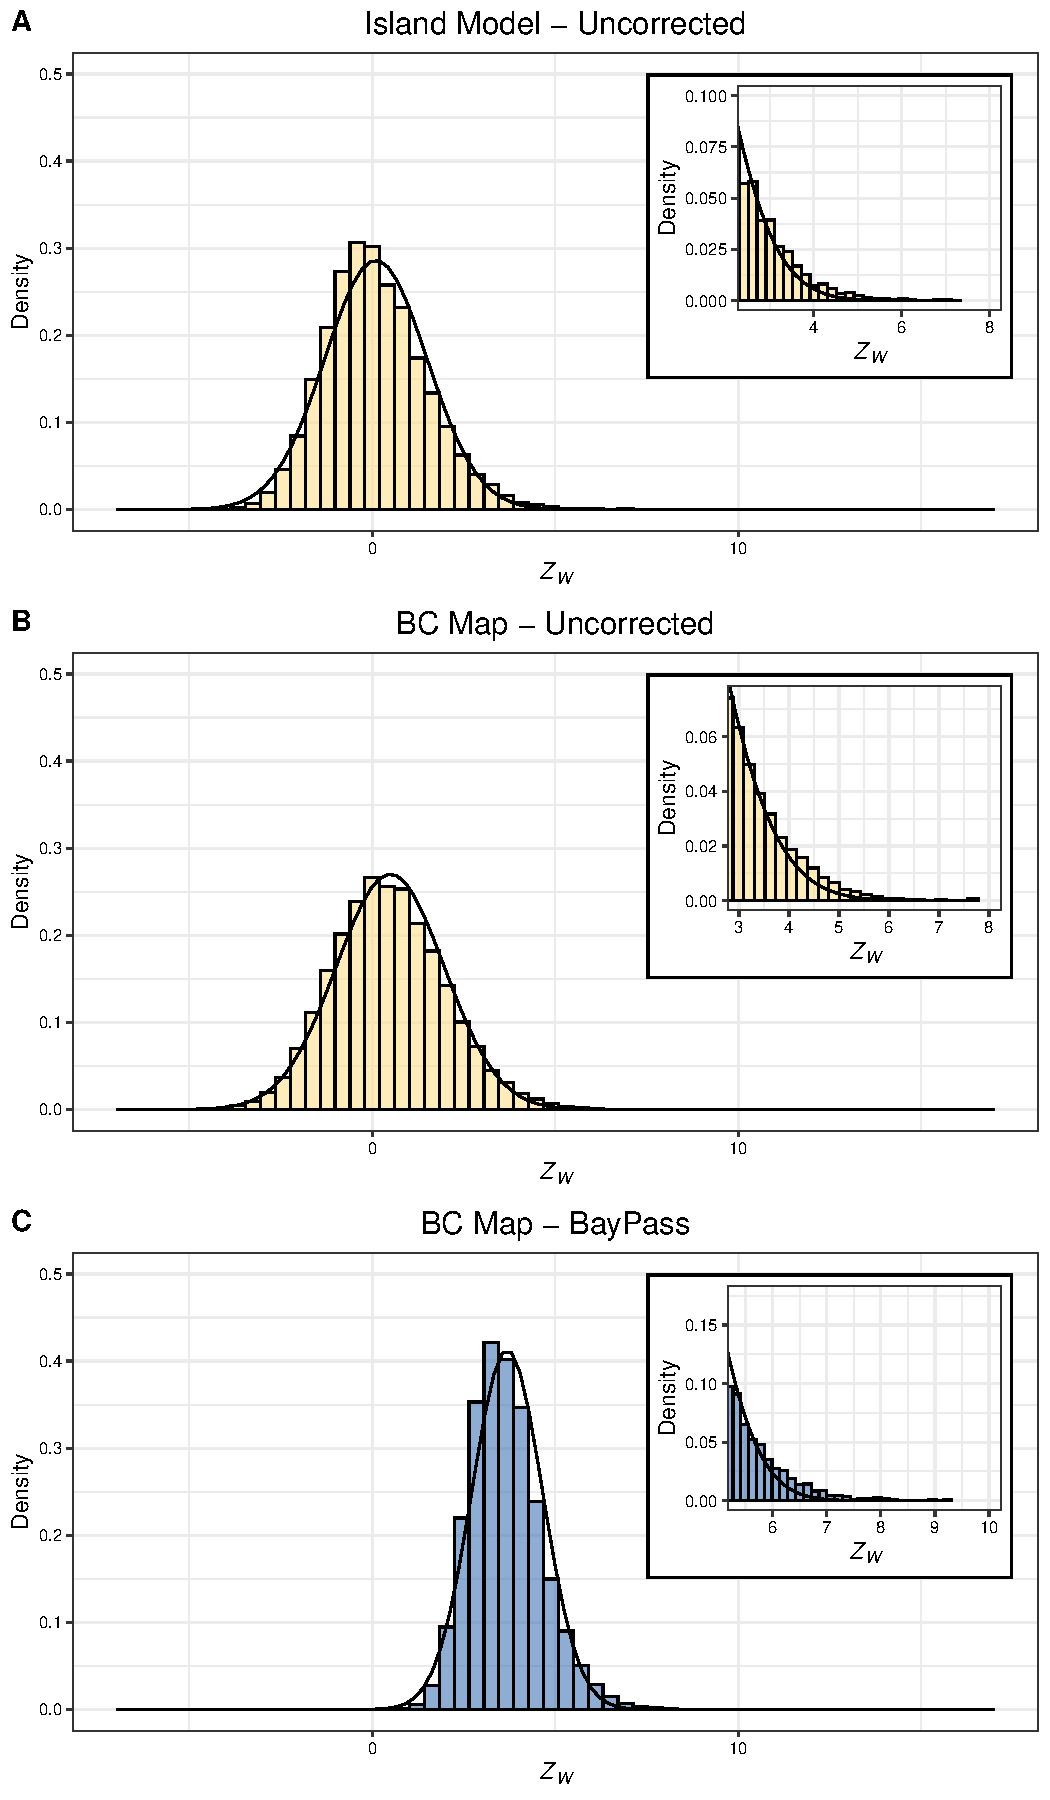
\includegraphics[height=0.5\linewidth,keepaspectratio]{Plots/neutralResults_histogram.pdf} 

  \caption{Density histograms of WZA scores for three cases. A) An finite island population, $Z_W$ scores were calculated using uncorrected $p$-values obtained from Kendall's $\tau$. B)  The BC-map, $Z_W$ scores were calculated using uncorrected $p$-values obtained from Kendall's $\tau$. C). Inset in each panel is a histogram focussing on the upper tail of the $Z_W$ distribution. The solid line in each panel is the normal distribution fit to the data.}
  
  \label{fig:NeutralHistograms}
\end{figure}

The WZA combines summary statistics from tests that are assumed to be statistically independent. Under the null hypothesis that all tests are non-significant, the distribution of the $Z_W$ is expected to be the standard normal distribution (i.e. a mean of 0 and a standard deviation of 1). In this study, we propose using the weighted-Z test to aggregate results for GEA studies applied to genome-wide SNPs. Tightly linked SNPs obviously violate the assumption of statistical independence, so the distribution of $Z_W$ scores from the WZA may not be normal. \\

To assess the statistical properties of the WZA, we first performed GEA analyses on populations structured according to an island model. While potentially unrealistic, the island model allowed us to determine the statistical properties of the WZA without spatial heterogeneity in the environment being confounded with population structure. We performed GEA using Kendall's $\tau$ on island model populations as if the data had been generated assuming the \textit{BC} map. Applying the WZA to GEA results for populations modelled under the island model, we found that the distribution of $Z_W$ scores slightly deviated from the null expectation; the mean $Z_W$ was 0.00X and the standard deviation was 1.XXX. Figure \ref{fig:NeutralHistograms}A shows the distribution of $Z_W$ scores was skewed with a fat right-hand tail.\\

We then applied the WZA to evolving neutrally stepping-stone populations and assumed the \textit{BC} map. The deviation from the null expectation of $Z_W$ scores was exaggerated when analysing data from stepping-stone simulations (Figure \ref{fig:NeutralHistograms}B-C). Figure \ref{fig:NeutralHistograms}B shows that the distribution of $Z_W$ assuming Kendall's $\tau$ results has a thicker right-hand tail than expected under the null. Applying the WZA to population structure corrected GEA (BayPass) results, we also found a thicker right hand tail to the distribution of $Z_W$ score than expected under the null. \\

If the distribution of $Z_W$ scores were normal, scores for particular genomic regions could be converted into \textit{p}-values. However, that the distribution was non-normal even when assuming the island model, suggests that linkage effects cause the deviation. Thus, we did use $Z_W$ scores to calculate parametric \textit{p}-vaues, rather, we used the $Z_W$ scores as an index for how much a particular genomic region deviates from the genome-wide pattern, similar to $F_{ST}$ calculated in analysis windows. \\

\subsection{Comparison of window-based and individual SNP-based GEA approaches}


\begin{figure*}
  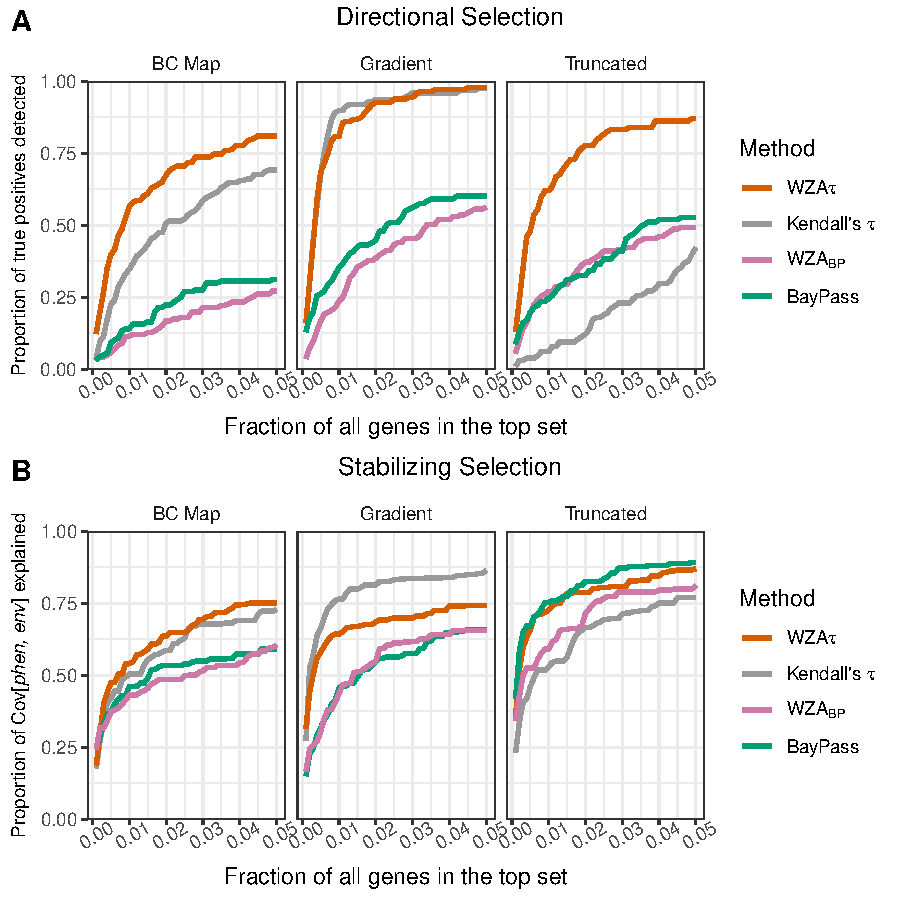
\includegraphics[width=0.6\linewidth]{Plots/UncorrectedBayPassComparison_TruePositives.pdf} 
  \caption{The proportion of true positives detected across a specified search effort when a model of local adaptation  by directional selection was assumed. A) shows results obtained from simulations assuming directional selection. B) shows results obtained assuming stabilising selection. Lines represent the mean of 20 simulation replicates. Note the different quantities on the y-axes.}

  \label{fig:truePosBoth}
\end{figure*}

We performed GEA on our simulated data using either Kendall's $\tau$, a rank correlation that does not model population structure, or \textit{BayPass} an analysis that attempts to estimate correlations between environmental variables and allele frequencies incorporating a population covariance matrix. Our simulations incorporated three different maps of environmental heterogeneity (Figure \ref{fig:envGridPlot}) and modelled local adaptation under either directional or stabilising selection. When using either \textit{BayPass} Bayes factors or \textit{p}-values from Kendall's $\tau$ as input to the WZA, the distribution of $Z_W$ scores for the genes that contributed to local adaptation separated from the distribution for neutrally evolving genes (Figure \ref{fig:ZScoreDistribution}). \\

To assess the performance of the WZA at identifying locally adaptive genes, we examined the distribution of test statistics from the WZA, the top-candidate method proposed by \citep{Yeaman2016}$Z_W$ scores in individual simulation replicates.



Figure \ref{fig:truePosBoth} shows how well the WZA, the top-candidate method and individual SNP approach perform when looking for the genes underlying local adaptation. There were notable differences in performance among the methods when simulations assumed directional or stabilising selection. Under directional selection, 
The biggest difference between \textit{BayPass} and the uncorrected approach was seen when assuming the \textit{Gradient} map. In that case, almost all of the true positives were detected when using the uncorrected \textit{p}-value approach whereas around 50\% were detected using \textit{BayPass} (Figure \ref{fig:truePosBoth}). \\

From Figure \ref{fig:falseDiscovery} it is clear that none of the GEA methods that we implemented are 


\begin{figure*}
  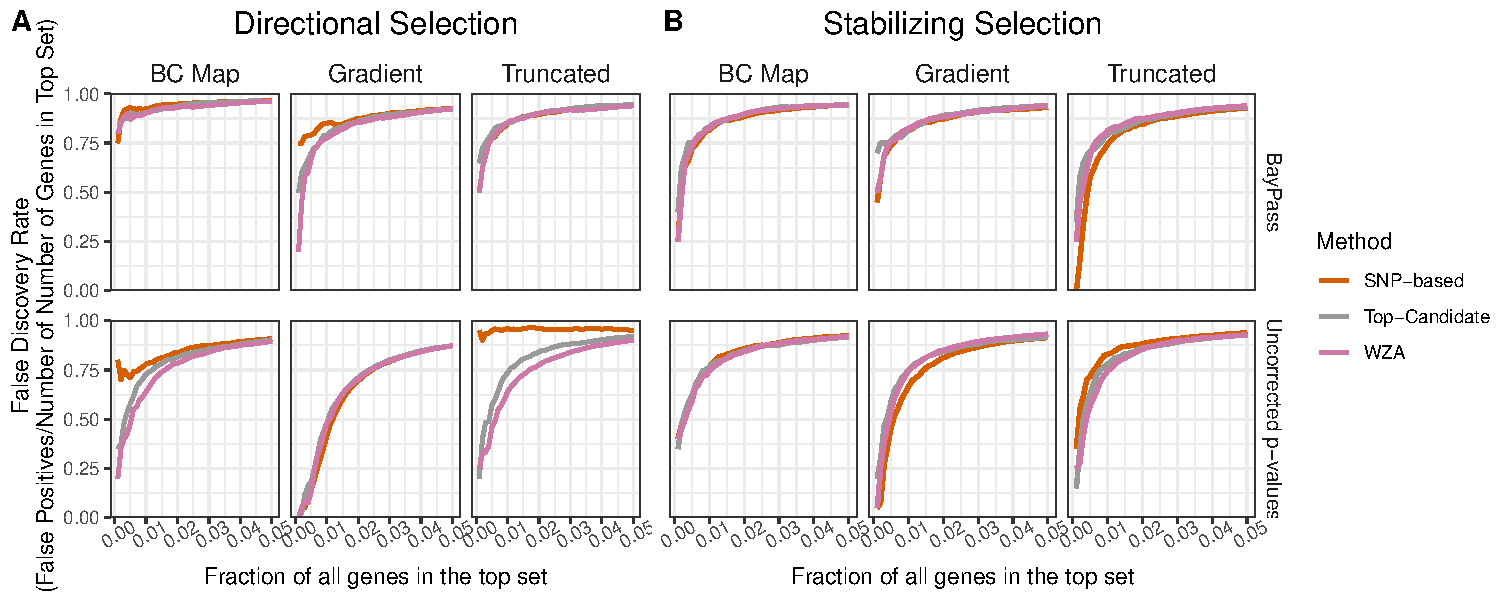
\includegraphics[width=0.6\linewidth]{Plots/UncorrectedBayPassComparison_FalsePositives.pdf} 
  \caption{The proportion of true positives detected across a specified search effort when a model of local adaptation  by stabilising selection was assumed.}

  \label{fig:falseDiscovery}
\end{figure*}



\subsection{The performance of WZA when GEA results are statistically noisy}
\textit{If either of you could come up with better sub-heading names, I'd be grateful}\\


The WZA is a method to aggregate data across linked sites to identify loci that exhibit a GEA pattern that deviates from the genomic background. The WZA is analogous to combining estimates of $F_{ST}$ for individual SNPs into analysis windows to identify signals in potentially noisy data \citep{Hoban2016}. For that reason, we postulated that the WZA would outperform the individual SNP approach when the underlying GEA was noisy. Here, we focus on three factors that may influence the ``noisiness" of a GEA study: 1) When the environmental variable in question is only partially correlated with the true selection pressure, 2) when GEA is applied to a relatively small number of demes and 3) when allele frequency estimates are based on a small number of individuals. \\
%As we had found that the uncorrected \textit{p}-value approach was more powerful than \textit{BayPass}, we focus on that test here.\\

Climatic or environmental variables may not be a perfect reflection of the selection pressures that species face in natural settings. It may be the case that a variable such as mean annual temperature is correlated with selection, but that that correlation is not perfect. Additionally, environmental variables likely include measurement error, contributing to an imperfect correlation with the true selection pressure. In the previous section, we conducted GEA assuming perfect knowledge of the phenotypic optima in each sampled deme. Here, we assess the performance of GEA methods when the measured environment (i.e. the 'E' in GEA) is not perfectly correlated with selection. We sampled data that were correlated with the true phenotypic optima to varying degrees and used them to perform GEA on the \textit{BC} map simulations. We assumed the simulations modelling stabilising selection and, as above, compared the performance of the WZA, top-candidate and the SNP-based GEA methods using \textit{BayPass} or Kendall's $\tau$. \\



\begin{figure*}
  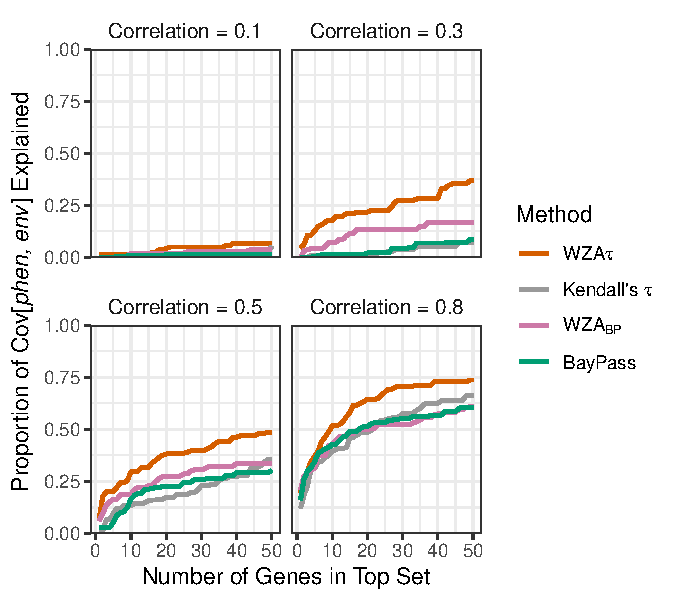
\includegraphics[width=0.6\linewidth]{Plots/correlatedEnvironments_BCmapResults.pdf} 
  \caption{The proportion of true positives recovered when the measured environment is correlated with selection pressure to varying degrees. The correlation between environment and selection pressure is shown above the plots. Results are shown assuming the BC Map and the model of stabilising selection.}

  \label{fig:truePosCorrelated}
\end{figure*}


We found that the window-based GEA methods outperformed single SNP approaches when the measured environment is not perfectly correlated with the true selection pressure. As might be expected, when the correlation between the measured environment and selection was very weak (i.e. a correlation of 0.1), few true positives were present in the top 50 genes with or without population structure correlation and those present explained only a small proportion of Cov(Phen. Env.)(Figure \ref{fig:truePosCorrelated}). With a correlation of 0.3 between the measured environment and true selection, the WZA substantially outperformed both the top-candidate method and single-SNP based approaches using BayPass or Kendall's $\tau$ (Figure \ref{fig:truePosCorrelated}). With a correlation of 0.5 or 0.8 between the measured environment and true selection, there were only small differences in performance between window-based and the single-SNP approaches when using BayPass (Figure \ref{fig:truePosCorrelated}). When using the uncorrected approach, however, the WZA and the top-candidate method outperformed the single-SNP approach (Figure \ref{fig:truePosCorrelated}). \\

In a hypothetical world where one had perfect knowledge of allele frequency variation across a species' range, a SNP-based approach would be the best way to perform a GEA analysis, as one would be able to determine the true correlation between genetic and environmental variation. Indeed, when one has perfect knowledge of allele frequencies, a SNP-based GEA outperforms the WZA and top-candidate methods for each of the maps we tested (Figure \ref{fig:sampleSize_demes}). However, such a situation is obviously unrealistic and  empirical GEA studies will likely always be limited to samples from population of interest. \\

So far we have only modelled a situation where 40 demes were sampled across the simulated metapopulations, with 50 individuals sampled in each location. We re-sampled the simulated populations, and extracted 50 individuals from 20 or 10 demes, the configuration of samples is shown in Figure \ref{fig:sampleMaps}. We compared the performance of the WZA to the top-candidate and SNP-based methods in these smaller datasets using the Kendall's $\tau$ \textit{p}-values. As expected, reducing the number of sampled demes from 40 to 20 or 10, reduced the proportion of true positives identified (Figure \ref{fig:sampleSize_demes}). However, we found that the WZA outperformed the top-candidate and SNP-based methods in datasets with 10 or 20 demes for each of the three maps we simulated (Figure \ref{fig:sampleSize_demes}).

In such cases, smaller numbers of demes and/or fewer individuals may be sampled. In either case, reducing sample sizes will reduce power of GEA, and potentially introduce statistical noise.
Indeed, reducing the number of sampled demes from 40 to 20 or 10 reduced the proportion of true positives detected across all analysis methods and maps of environmental heterogeneity (Figure REFERENCE). Notably, though, the WZA outperformed the top-candidate and SNP-based method when the  

We compared the performance of the WZA to the top-candidate and SNP-based methods when a fewer than 40 demes were sampled. Reducing the number of sampled demes reducedFigure XXX shows 

\subsection{Application of the WZA to data from lodgepole pine}

We re-analysed a previously published \citep{Yeaman2016} lodgepole pine (\textit{Pinus contorta}) dataset comprising 256 populations sampled across North Western North America.\cite{Yeaman2016} performed GEA on their data using numerous environmental variables, but here we only analyse DD0. \cite{Yeaman2016} phenotyped the lodgepole pine populations they studied for response to injury from freezing temperatures. They found that the cold-injury response phenotype for a population was strongly negatively correlated with the estimated DD0, suggesting that DD0 is correlated with a true local adaptation pressure. \\

We downloaded the data associated with the \cite{Yeaman2016} study, which included tables containing allele frequency and GEA results (Spearman's $\rho$ and the associated \textit{p}-value) for genome-wide SNPs. \cite{Yeaman2016} applied the top-candidate method to these data. Here, we replicated that analysis but also applied the WZA, using genes as the unit of analysis. Unlike our analysis of simulation data, where we divided the genome into analysis windows of a fixed physical size, \cite{Yeaman2016} analysed gene sequences. \\

Across the lodgepole pine genome, $Z_W$ scores had a mean of 0.013 and $\sigma = 1.67$. Additionally, the distribution of $Z_W$ had a fat right-hand tail (Figure \ref{fig:lodgepoleDescriptives}B). Figure \ref{fig:lodgepole}A shows the relationship between WZA scores and the $-log_{10}(p-values)$ from the top-candidate method. The scores from the two tests were positively correlated (Kendall's $\tau$ = 0.245, \textit{p}-value < $10^{-16}$). Figures \ref{fig:lodgepole}C-D show the relationship between allele frequency and the empirical \textit{p}-value for SNPs present in two genes that had extreme scores from both the top-candidate method and the WZA. There were several genes that had $Z_W$ scores greater than 10 (approximately $6\sigma$), but very modest top-candidate scores (Figure \ref{fig:lodgepole}A). Figure \ref{fig:lodgepole}B shows that for one such region, there were several SNPs with high mean allele frequency that have small \textit{p}-values. This particular region had a high \textit{p}-value from the top-candidate method. Conversely, Figure \ref{fig:lodgepole}C shows a region that only had a $Z_W\approx5$, but an extremely small \textit{p}-value from the top-candidate method. In this case, there were numerous SNPs that passed the top-candidate significance threshold, but they were mostly at low allele frequency.
\begin{figure}[H]
  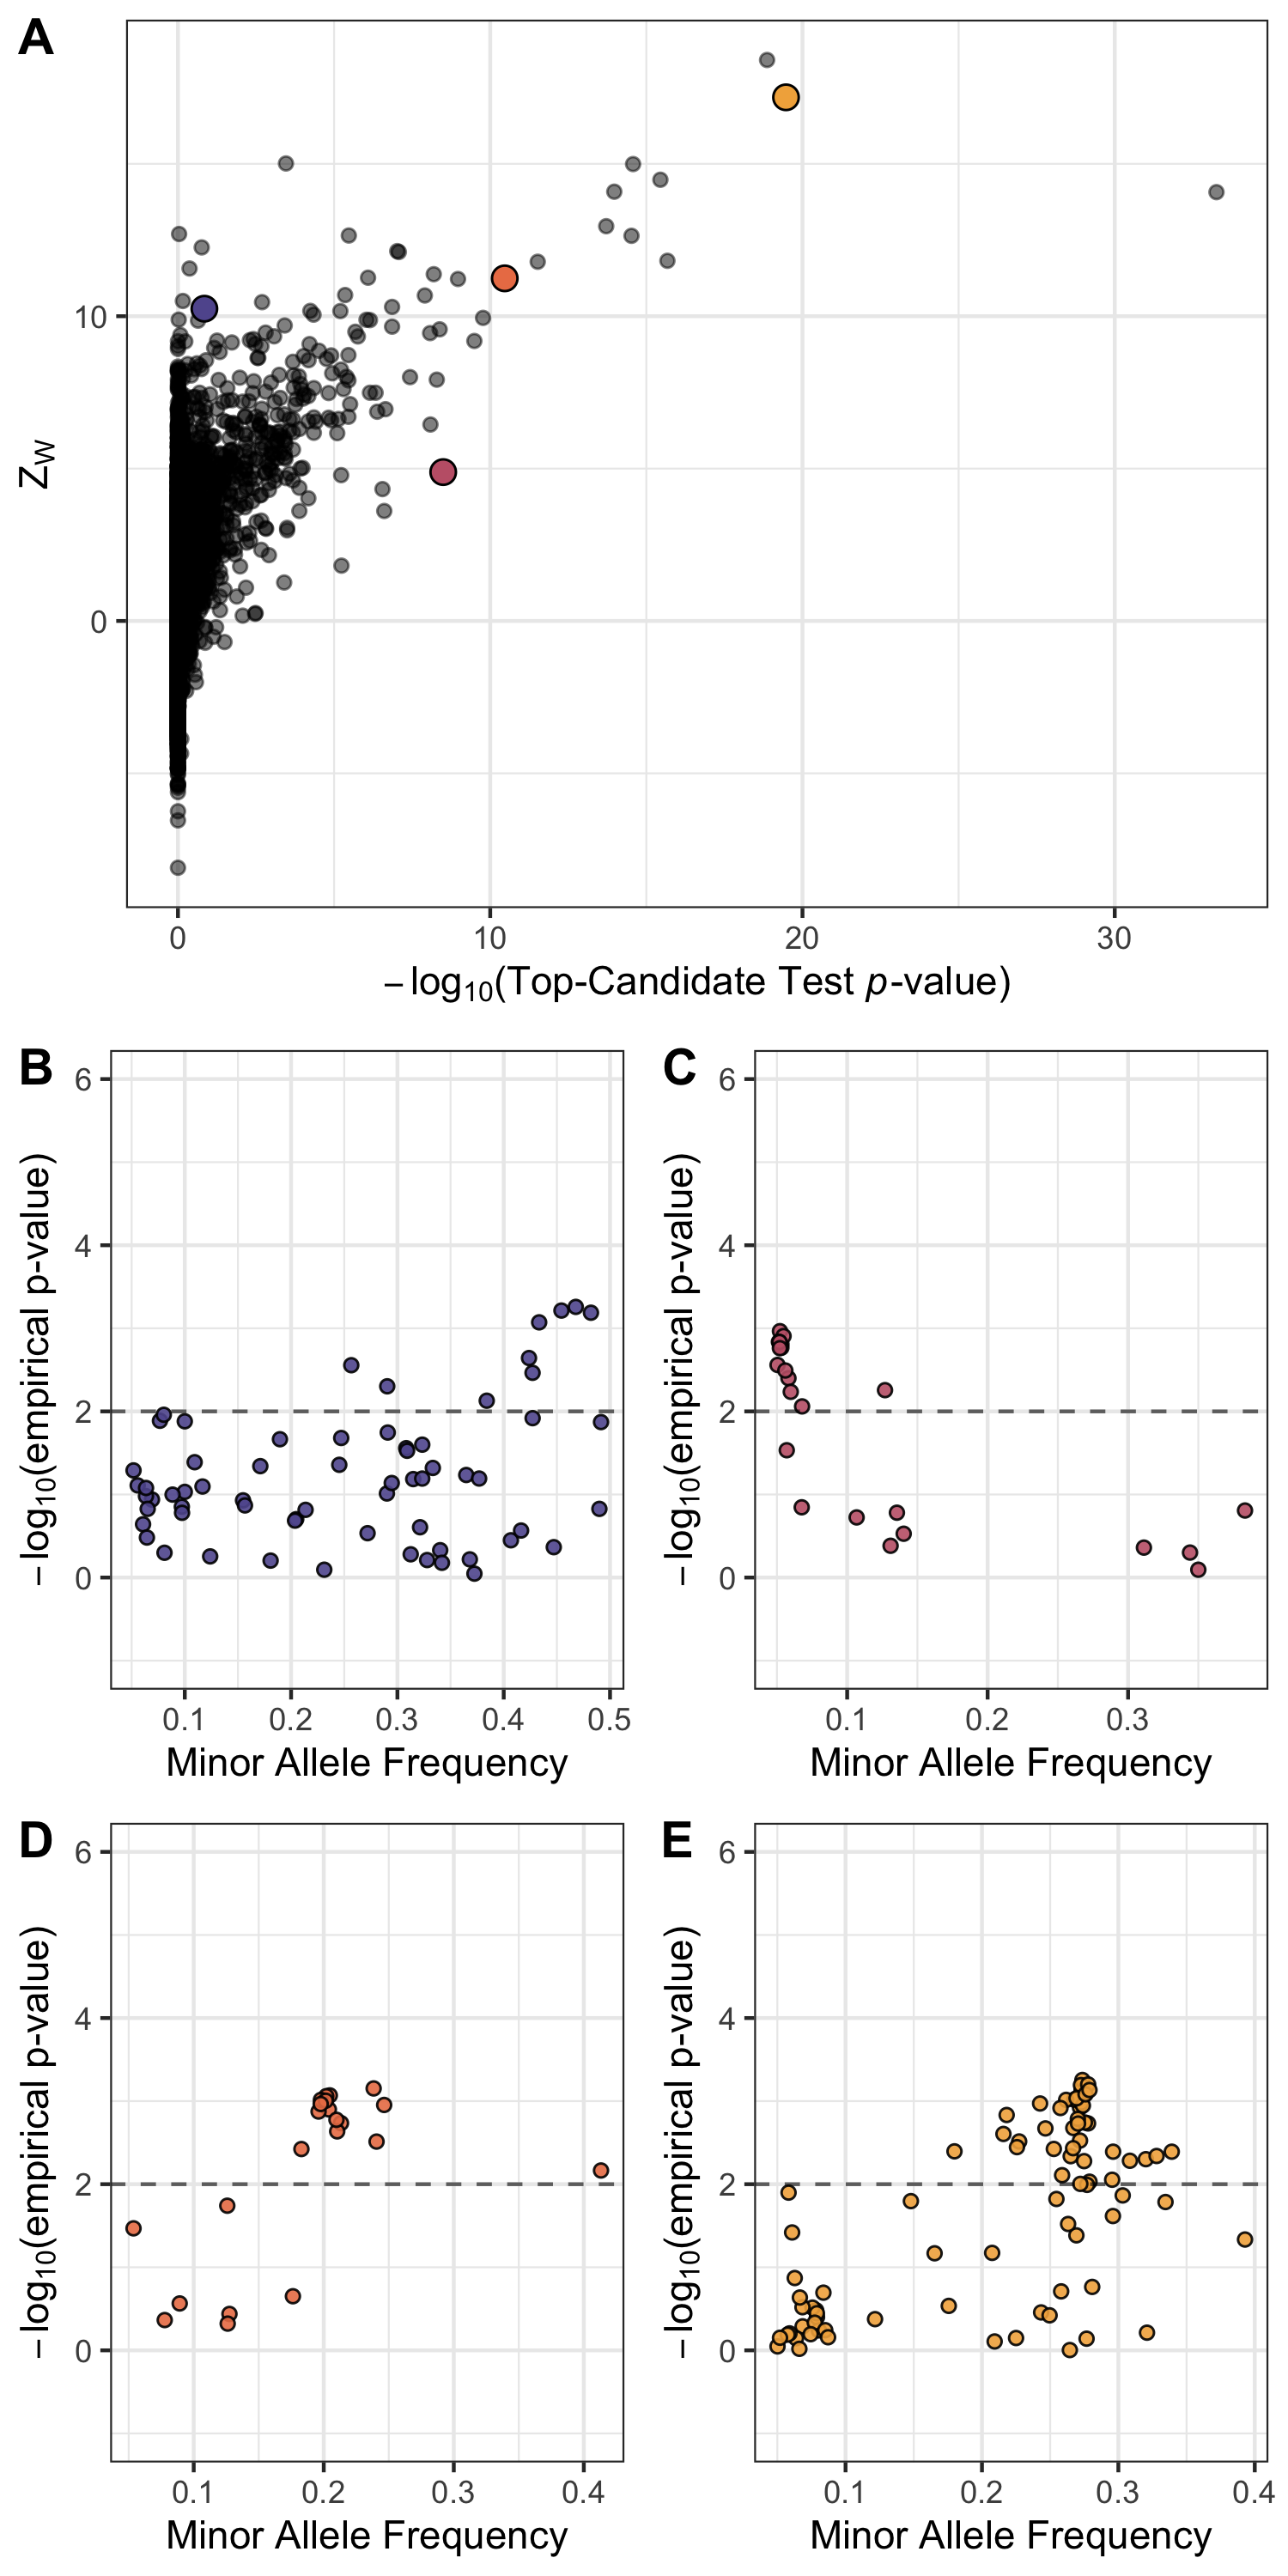
\includegraphics[width=0.75\textwidth,height=0.75\textheight,keepaspectratio]{../dataAnalsis/Z_v_MAF_DD0.png}
  \caption{The WZA applied to GEA results Lodgepole Pine for degree days below 0 (DD0). A) $Z_w$ scores compared to scores from the top-candidate method for each of the genes analysed by \cite{Yeaman2016}. Panels B-E show the results for $-log_{10}$(\textit{p}-values) for Spearman's $\rho$ applied to individual SNPs against minor allele frequency (MAF). The dashed horizontal line in B-D indicates the significance threshold used for the top-candidate method (i.e. $99^{th}$ percentile of GEA $-log_{10}$(\textit{p}-values) genome-wide).}

  \label{fig:lodgepole}
\end{figure}


%%%%%%
%      % 
%       % 
%       % 
%       % 
%       %
%       %
%       %
%     %
%%%%%%

\section{Discussion}

In this study, we have shown that combining information across linked sites in GEA analyses is a potentially powerful way to identify genomic loci involved in local adaptation. The method we propose, the WZA, was often more powerful than looking at individual sites in isolation, particularly when working with small samples or when the environmental variation being analysed is only weakly correlated with selection. An advantage of the WZA is that it provides a continuous metric that naturally lends itself to comparison among species. For example, one could compare $Z_W$ scores for a particular genes that were orthologous among distantly related species as a way to identify convergent evolution.  \\
%However, even if GEA methods are underpowered in a particular system, the distribution of $Z_W$ scores for genes involved in local adaptation had a higher mean than the non-adapted genes when we simulated stabilising selection (Figure \ref{fig:ZScoreDistribution}, which included many loci of small effect (Figure \ref{fig:effectSizeDistribution}), so while it may be very difficult to distinguish locally adaptive loci in such cases, gene ontology enrichment anal 
%even if specific loci might be ficcicult to identify, gene ontology analysis . 

In many of the cases we examined, the performance of the WZA and the top-candidate method of \cite{Yeaman2016} were fairly similar (Figure \ref{fig:truePosBoth}). However, there are philosophical reasons as to why the WZA should be preferred over the top-candidate method. First, the top-candidate method assumes that there is a fraction of genetic markers analysed that are tagging causal variants (i.e. that there are true positives in the dataset). This is undesirable, however, because genuine genotype-environment correlations may be very weak and GEA may simply be an underpowered approach to identify alleles that contribute to local adaptation. If there were no detectable signal of local adaptation, ascribing significance to a fraction of the genome may lead to false positives. Secondly, the top-candidate method gives equal weight to all SNPs that have exceeded a fixed significance threshold. For example, with a significance threshold of \textit{$\alpha$} = 0.01, genomic regions with only a single outlier are treated in the same way whether that outlier has a \textit{p}-value of 0.009 or $10^{-10}$. It seems desirable to retain information about particularly strong outliers. \\

It should be kept in mind that the WZA (and the top-candidate method for that matter) does not explicitly test for local adaptation and only provides an indication of whether a particular genomic region has a pattern that deviates from the genome-wide average. Indeed, numerous processes other than local adaptation may cause excessive correlation between environmental variables and allele frequencies in particular genomic regions. For example, population expansions can cause allelic surfing, where regions of the genome ``surf" to high frequency at leading edge of an expanding population. Allelic surfing can leave a heterogeneous patterns of variation across a species range leaving signals that may resemble local adaptation \citep{Novembre2009, Klopfstein2006}.  \\

As stated above, a feature of the WZA is that a wide range of summary statistics could be used as input. We converted \textit{p}-values from Kendall's $\tau$ correlation or Bayes factors from \textit{BayPass} into empirical \textit{p}-values and used these as input to the WZA. The use of empirical \textit{p}-values to account for genome-wide false positives is not unique to this study, we got the idea from \cite{Hancock2011} who used empirical \textit{p}-values from GEA results to identify loci involved in climate adaptation in \textit{Arabidopsis thaliana}. While the empirical \textit{p}-value approach corrects for false positives due to population structure genome-wide, it throws away the null model for our summary statistic of interest. A GEA approach that produced parametric \textit{p}-values that was adequately controlled for population structure may provide a more powerful input statistic to the WZA. Alternatively, with the advent of methods for reconstructing ancestral recombination graphs from population genomic data \citep{Hejase2020}, perhaps a GEA method could be developed that explicitly analyses inferred genealogies rather than individual markers in a manner similar to regression of phenotypes on genealogies proposed by \cite{Ralph2020}. \\

%Something about population structure approaches:


%If the hypothetical species had restricted migration and exhibited isolation-by-distance, neutral alleles may be correlated with environmental variables that happen to correlate with latitude simply due to population structure. For that reason, any attempt to identify loci involved in adaptation may then be stymied by an underlying correlation between presumed selection pressures and directions of gene flow; \cite{Sohail2019} and \cite{Berg2019} provide a clear example of this problem in an analysis of selection on human height. GEA approaches may correct for population demography when calculating correlations with the environment

\subsection{The width of analysis windows}

When performing a genome scan using a windowed approach a question that inevitably arises is, how to to decide on the width of analysis windows? In our simulation study, we used analysis windows that were 10,000bp long and within that distance LD had fully decayed to background levels (Figure \ref{fig:summaryStats}). LD can be considered as the correlation in coalescence times between pairs of sites (McVean 2002; Wakeley 2007), so high LD is suggestive of highly correlated evolutionary histories. If the width of an analysis window were greater than the average distance over which LD decayed the window would presumably encompass a variety of evolutionary histories, some more correlated than others. Applying the WZA to GEA results in 10,000bp windows in our analysis of simulated data led to a distribution of $Z_W$ scores that was close to the null expectation of the standard normal distribution, but with a thicker right hand tail (Figure \ref{fig:NeutralHistograms}). The deviation from normality presumably arose because some SNPs in the analysis windows had highly correlated histories, violating the independence assumption of the weighted-Z test. 

On the other hand, if analysis windows were narrower than the average distance over which LD decayed most SNPs would presumably have highly correlated evolutionary histories. Random drift may cause genealogies in some regions of the genome to correlate with environmental variables more than others. Many of the SNPs present in an analysis window that consisted of genealogies that were highly correlated with the environment may be highly significant in a GEA analyses, leading to a large $Z_W$ value. This effect would lead to a larger variance in $Z_W$ for analysis windows that were narrower than the average LD decay. We down sampled the tree-sequences we recorded for our simulated populations to model analysis windows present in low recombination regions and performed the WZA on the resulting data. As expected, we found that the variance of the distribution of $Z_W$ scores was greater when there was a lower recombination rate (Figure \ref{fig:WZA_Recombination}). \\

Theoretical studies of local adaptation suggest that we should expect regions of the genome subject to spatially varying selection pressures to exhibit elevated linkage disequilibrium (LD) relative to the genomic background for a number of reasons. Under local adaptation, alleles are subject to positive selection in some parts of a species's range, but not in others. As a locally adaptive allele spreads in the locations where it is beneficial, it may cause some linked neutral variants to hitchhike along with it \citep{Sakamoto2019}. Non-beneficial genetic variants introduced to local populations via gene flow may be removed, with a result being a build up of LD between selected alleles and linked neutral sites. This process can be thought of as a local barrier to gene flow \citep{Barton1986}. Beyond this hitchhiking signature, there is a selective advantage for alleles that are involved in local adaptation to cluster together, particularly in regions of low recombination \citep{Rieseberg2001, Noor2001, Kirkpatrick2006, Yeaman2013}. For example, in sunflowers and \textit{Littorina} marine snails, there is evidence that regions of suppressed recombination cause alleles involved in local adaptation to be inherited together \citep{Morales2019, Todesco2020}. The processes we have outlined are not mutually exclusive, but overall, genomic regions containing strongly selected alleles that contribute to local adaptation may have elevated LD and potentially exhibit GEA signals at multiple linked sites.\\

Window size would ideally be informed by the extent by which LD decays at neutral sites and how much LD is induced by selection. Determining that is likely very difficult however as understanding the effects of migration-selection balance on linkage disequilbrium requires estiamtes of selection and dispersal which are difficult to determine. Additionally, recombination rates vary widely among taxa but also within the genome \citep{Stapley2017}. Such variation causes LD to decay over greater or shorter distances in different locations across the genome so window size may need to be dynamic with respect to recombination rate variation. Random drift may cause some regions of the genome to correlate with environmental variables more than others. If such drift happens in regions of low recombination, multiple linked SNPs may exhibit strong GEA signals. This would lead to a distribution of $Z_W$ scores that had a higher variance in regions of low recombination and generate statistical artefacts as we outlined in our previous study \citep{Booker2020}. 



\section{Acknowledgements}

Thanks to Pooja Singh for many helpful discussions, to Tongli Wang for help with BC climate data and to Simon Kapitza for help with wrangling raster files. Thanks to Finlay Booker for moral support throughout the course of this project. TRB is supported by funding from Genome Canada, Genome Alberta and NSERC Discovery Grants awarded to MCW and SY. SY is supported by an AIHS research chair and NSERC Discovery Grant. MCW is supported by an NSERC Discovery Grant. Computational Support was provided by Compute Canada.\\

\bibliography{references}

\beginsupplement
\onecolumn
\section{Appendix}

\section{Parametrising simulations of local adaptation}
Consider a hypothetical species of conifer inhabiting British Columbia. There may be many hundreds of millions of individuals in this hypothetical species distributed across the landscape. It would be computationally intractable to simulate all individuals forward-in-time, incorporating adaptation to environmental heterogeneity across the landscape and recombining chromosomes. In our simulations we scaled several population genetic parameters to model a large population when simulating a much smaller one. In the following sections, we outline and justify the approach we used to scale pertinent population genetic parameters. 

\subsection{Mutation rate} 
The neutral mutation rate was set such that there would be an average of around 30 SNPs that had  a minor allele frequency greater than 0.05. We aimed at around 20-30 SNPs per gene as that is the number identified for lodgepole pine by \cite{Yeaman2016}. 

\subsection{Recombination rates}
In conifers, recombination rates ($r$) have been estimated to be on the order of 0.05 cM/Mbp; more than 10$\times$ lower than the average for humans \citep{Stapley2017}. The pattern of LD decay in a panmictic population can be predicted by the population scaled recombination parameter ($\rho = 4N_er$; \citealt{RN173}), but the pattern of LD decay in structured is less well described. However, LD decays very rapidly in conifers \citep{Pavy2012}. In conifers, $\rho = 0.005$ has been estimated \citep{Pavy2012}. This implies a very large effective population size of roughly $\frac{0.005}{4\times0.5\times10^{-8}} = 2.5 \times 10^6$, much larger than is feasible to simulate. We simulated meta-populations of 19,600 individuals 

We thus chose a recombination rate that gave us a pattern of LD decay that was similar to what has been observed in conifers. We set the per base pair recombination $r = 1 \times 10^{-7}$.

to simulate populations with a recombination rate parameter of $4N_dr = 0.00004$ as we found this gave a pattern of LD-decay in our stepping-stone populations (Figure \ref{fig:summaryStats}). Note that the 
	that was very similar to what has been observed in conifers. To achieve levels of LD-decay in our simulations that are similar to those expected in our hypothetical organism, we set $4N_dr = 0.00004$, but with only 100 individuals per deme that gave a per base pair recombination of $1 \times 10^{-7}$.

\subsection{Selection coefficients} 

It is difficult to choose a realistic set of selection parameters for modelling local adaptation because there are, at present, no estimates of the distribution of fitness effects for mutations that have spatially divergent effects. However, common garden studies of a variety of taxa have estimated fitness differences of up between 35-45\% between populations grown in home-like conditions versus away-like conditions \citep{Hereford2009, Bontrager2020}. Motivated by such studies, we chose to parametrise selection using the maximum possible fitness difference between home versus away environments.\\

When modelling directional selection, our simulations contained 12 loci that could mutate to generate a locally beneficial allele. The phenotypic optima that we simulated ranged from -7 to 7 and we modelled selection on a locus as $1 + s_a\theta$ for a homozygote and $1 + hs_a\theta$ for a heterozygote, where $s_a$ is the selection coefficient, $\theta$ is the phenotypic optimum and $h$ is the dominance coefficient. With a selection coefficient of $s_a = 0.003$, the maximum relative fitness was $(1+7\times s_a)^{12} = 1.28$ for an individual homozygous for all locally beneficial alleles. An individual homozygous for those alleles, but in the oppositely selected environment (i.e. present in the wrong deme) had a fitness of $(1-7\times 0.003)^{12} = 0.775$. However, in preliminary simulations, we found that directional selection on locally beneficial alleles with $s_a = 0.003$ resulted in such strong patterns of local adaptation that all GEA methods identified all adapted loci with ease. We thus chose to reduce the strength of selection in the directional selection simulations to $s_a = 0.003$, this resulted in a maximum of 35\% difference in fitness between individuals grown in home-like conditions versus away-like conditions.

As stated the main text, for stabilising selection simulations we chose $V_s = 192$ as this gave a maximum of 50\% difference in fitness between individuals grown in home-like conditions versus away-like conditions.

\subsection{Migration rate} 
For the migration rate, we worked backwards. We set out to achieve $F_{ST}$ across the metapopulation of approximately 0.05, as has been reported for widely distributed conifer species such as lodgepole pine and interior spruce \citep{Yeaman2016}. For the stepping-stone simulations, we chose a migration rate of $\frac{7.5}{2N_d}$ as we found that this gave a mean $F_{ST}$ of 0.04. For an island model, we used the analytical formulae given in the main text to set $m$ to achieve a mean $F_{ST}$ of 0.03. 

\pagebreak

\begin{table}[H]
\label{tab:SimulationParameters}
\caption{Population genetic parameters of a hypothetical organism, and how they are scaled in the simulations. The meta-population inhabits a $14\times14$ 2-dimensional stepping stone. Parameters are shown for a population with 12 loci subject to directional selection.}
\begin{tabular}{lcccl}
\cline{1-4}
\textbf{Parameter} & \textbf{Hypothetical Biological Value} & \textbf{Scaled Parameter}        & \textbf{Unscaled (simulation)} \\ \cline{1-4}
Global population size ($N_e$)                 & $10^6$                                      & -                           & 19,600                                              &           \\
Number of demes ($d$)                  & 196                                      & -                           & 196                                                &           \\
Local population size ($N_d$)                  & 5,100                                      & -                           & 100                                                &           \\
Recombination rate (\textit{r})                        & $10^{-8}$                                      & $4N_dr = 2.04 \times 10^{-4}$ & $5.10 \times 10^{-7}$                                           &           \\
Selection coefficient (\textit{$s_{Max}$})                        & 0.0001                                         & $2N_ds_{Max}= 0.6$ & 0.003                                           &           \\
Migration rate (\textit{m})                        & $9.80\times 10^{-4}$                                      & $2N_dm = 10$        & 0.05                                               &           \\
Functional mutation rate (\textit{$\mu_\alpha$})                        & $2\times 10^{-10}$                                      & $4N_e\mu_\alpha = 0.0008$        & $10^{-8}$ &           \\ \cline{1-4}
\end{tabular}

\end{table}

\pagebreak

\begin{figure}[H]
  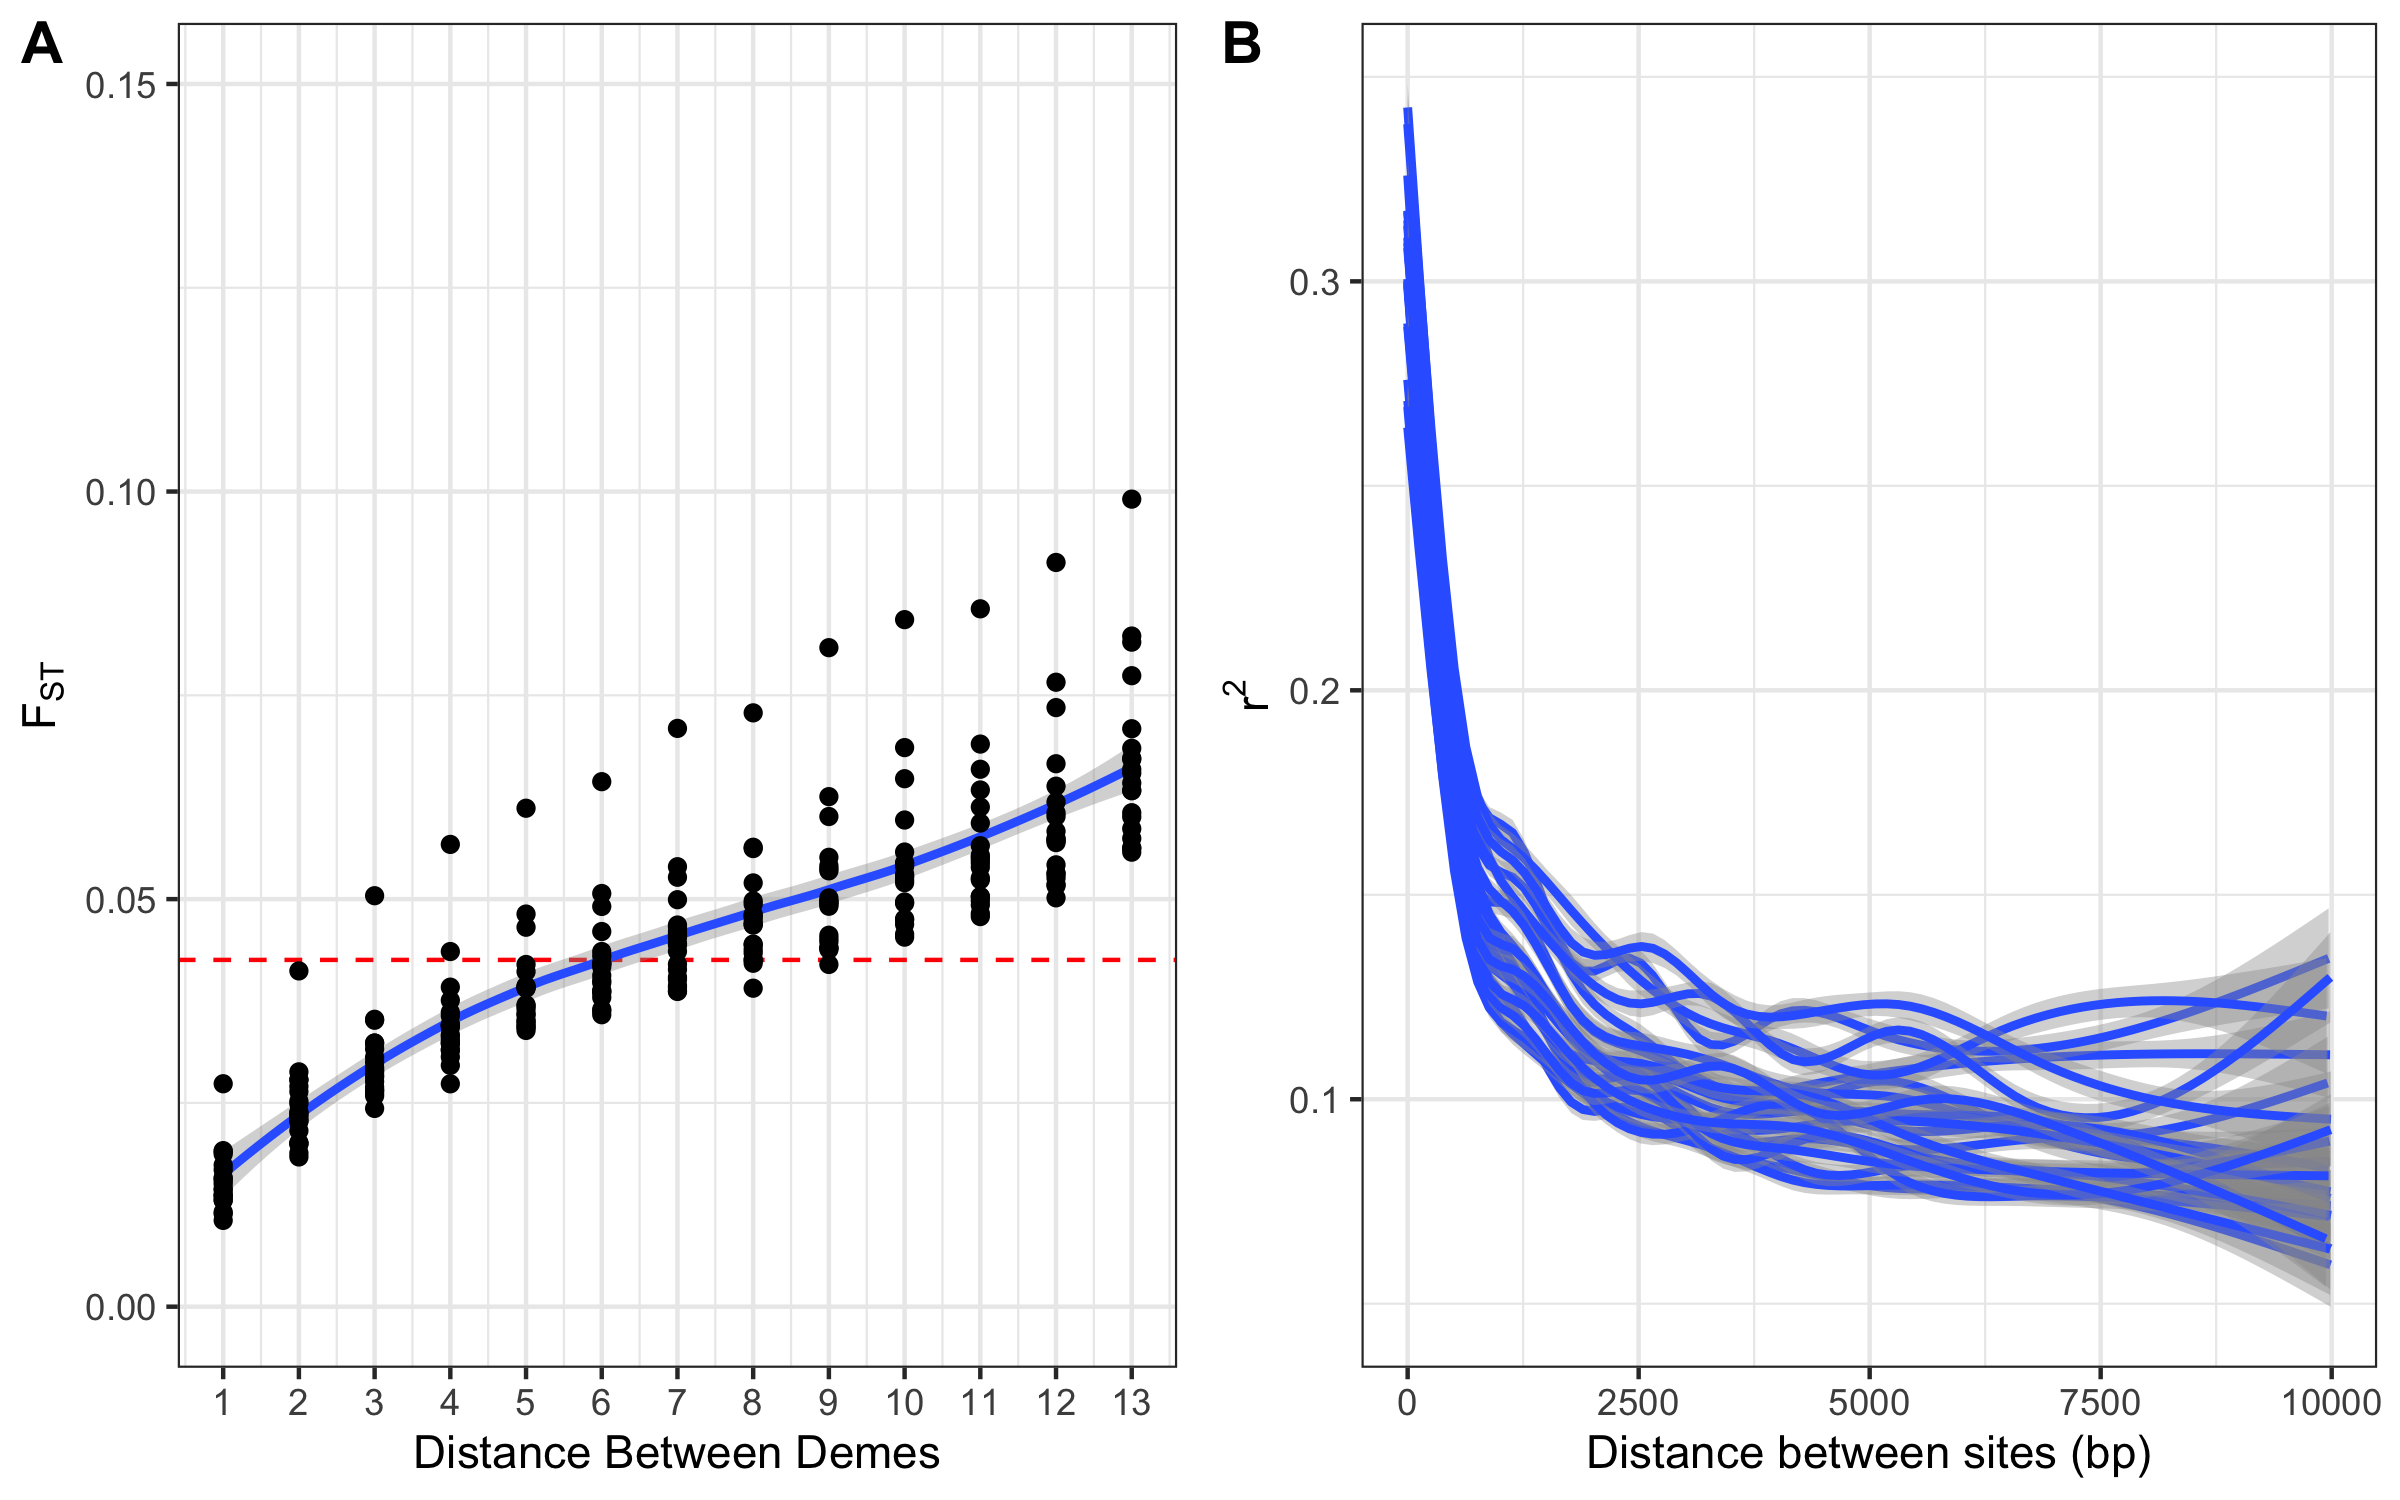
\includegraphics[width=\textwidth,height=0.75\textheight,keepaspectratio]{../SimulationStudy/directionalSelection/SummaryStats.png}
  \caption{Summary statistics from simulations. A) shows the $F_{ST}$ between pairs of demes in stepping-stone populations, the average across replicates is . B) shows LOESS smoothed LD, as measured by $r^2$, between pairs of SNPs, each line corresponds to a single simulation replicate.}

  \label{fig:summaryStats}
\end{figure}

\pagebreak

\begin{figure}[H]
  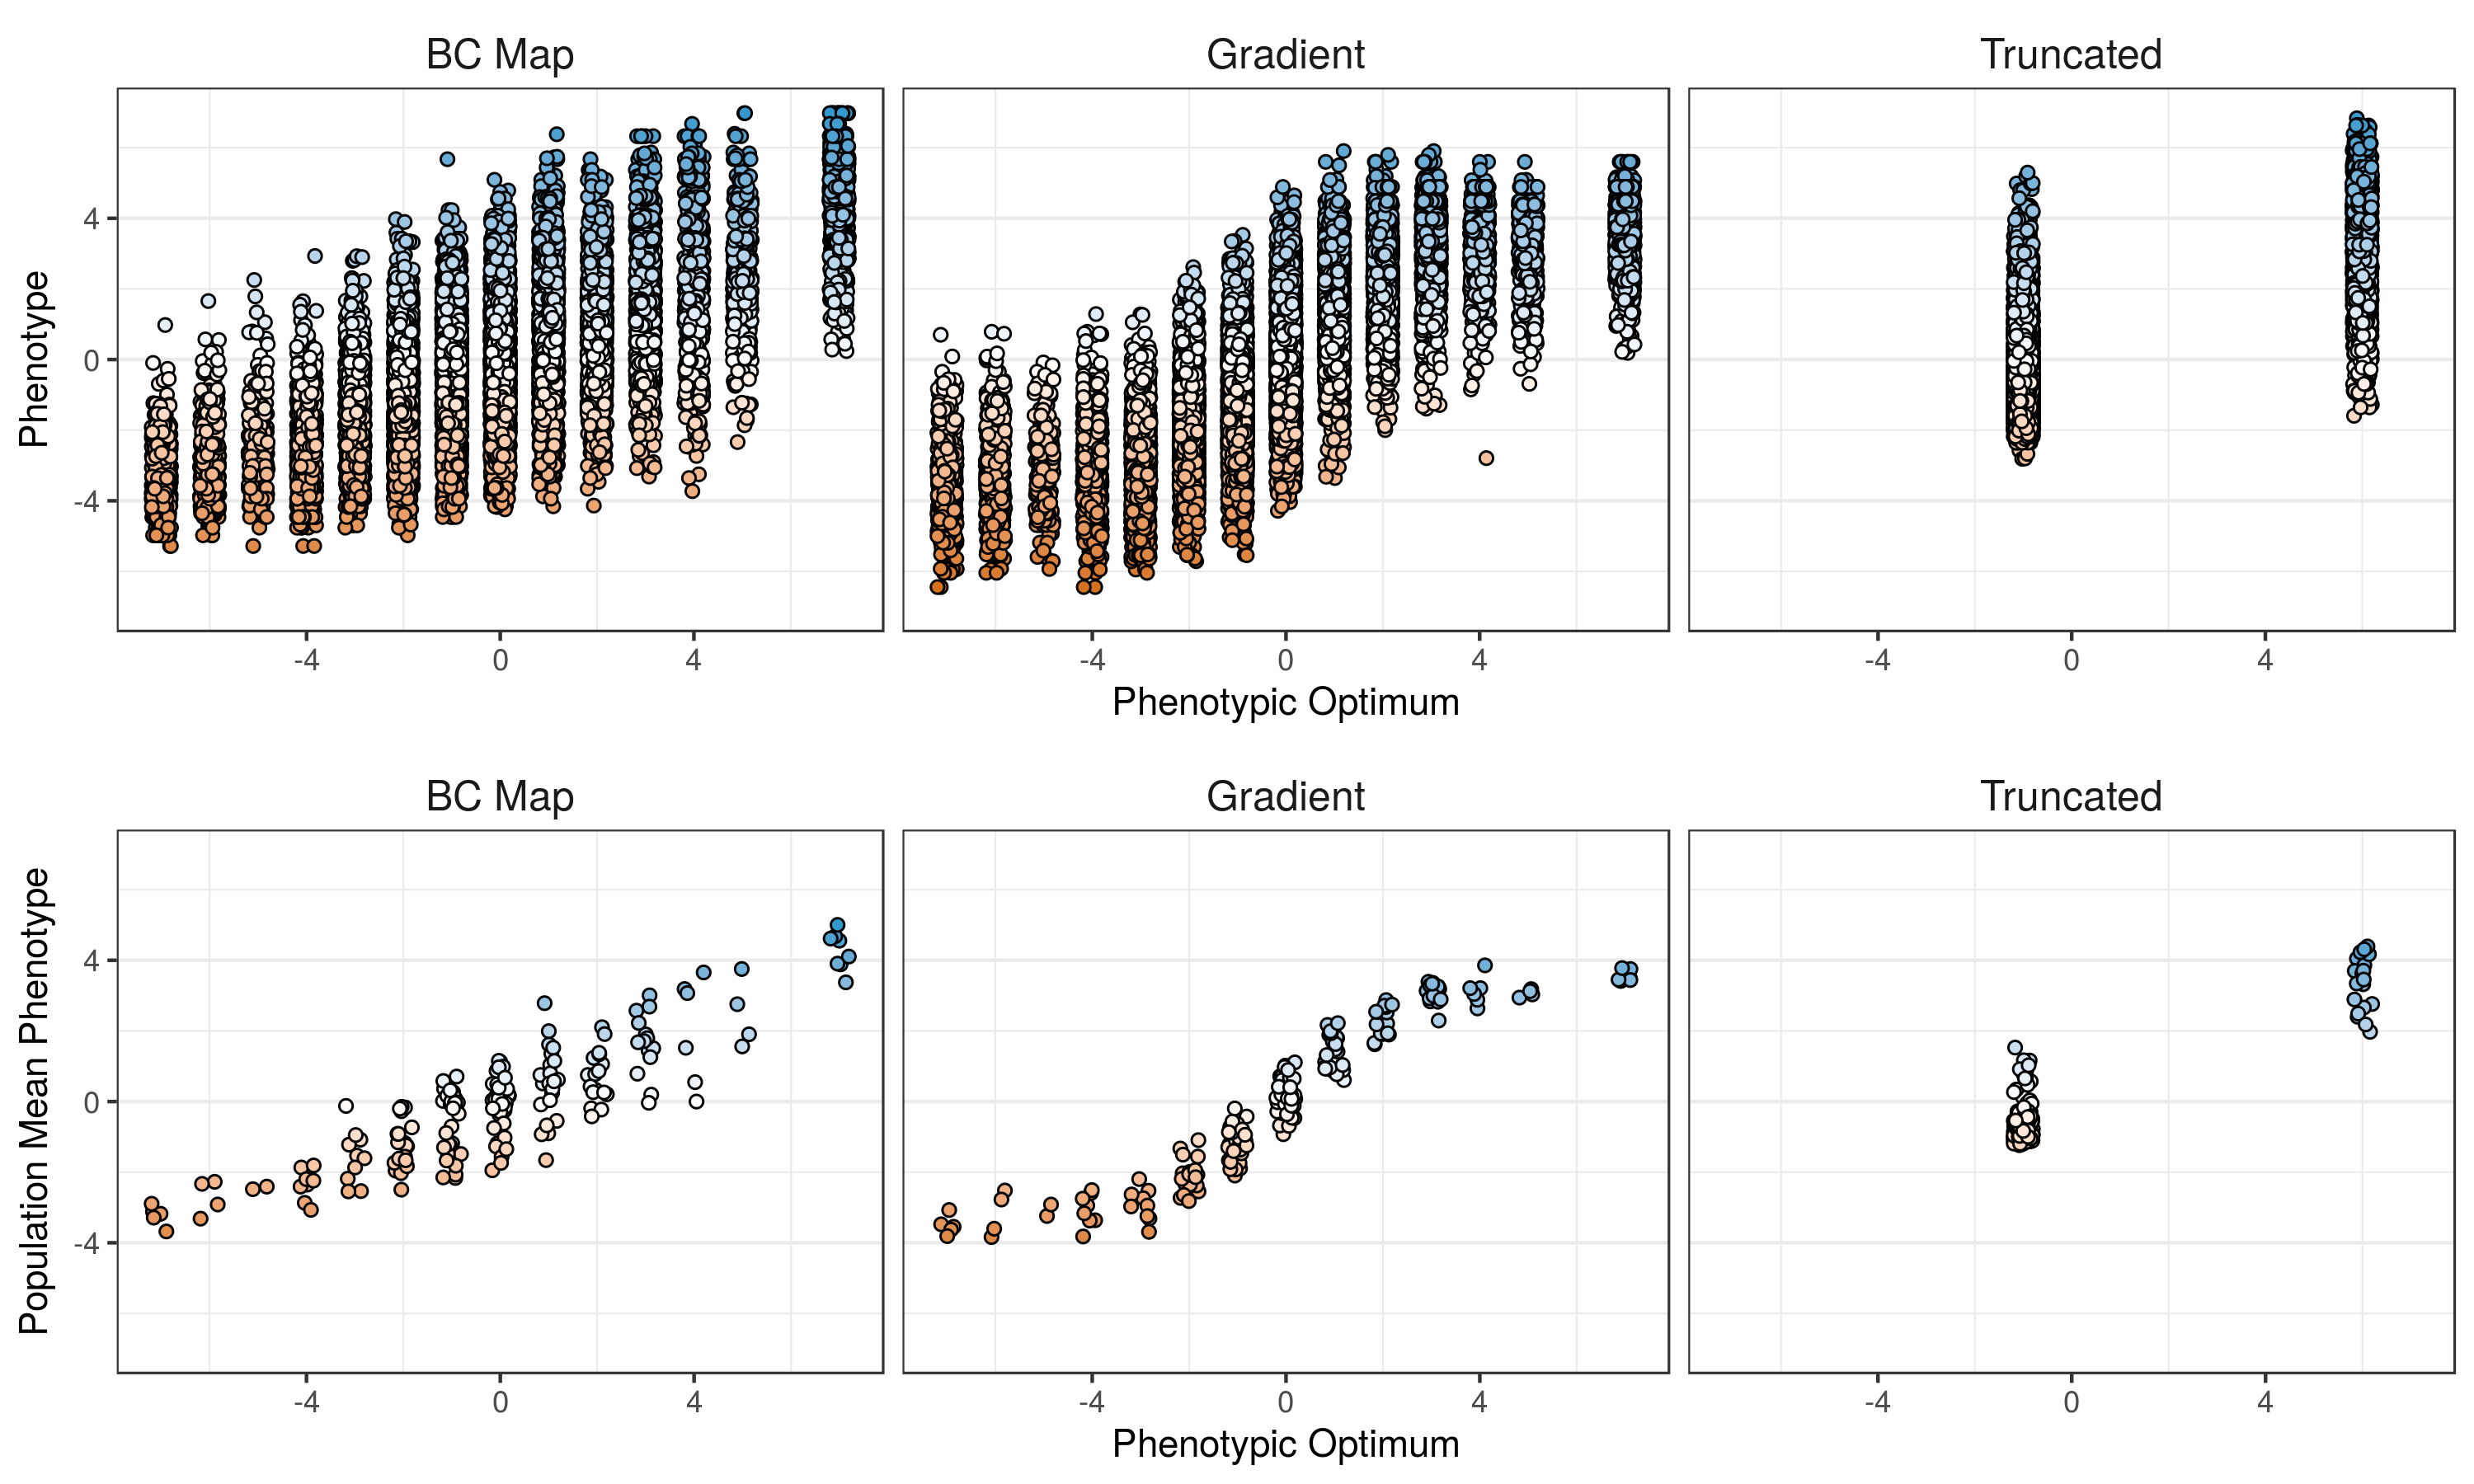
\includegraphics[width=\textwidth,height=0.75\textheight,keepaspectratio]{Plots/PhenotypePlot.png}
  \caption{Individual and population mean phenotypes observed in representative simulations for each of the environment maps simulated. A small amount of horizontal jitter was added to points for visualisation purposes}

  \label{fig:localAdaptationPhenotypes}
\end{figure}

\pagebreak


\begin{figure}[H]
  \includegraphics[width=\textwidth,height=0.75\textheight,keepaspectratio]{Plots/effectSizeDistributionPlot.pdf}
  \caption{The effect size distribution from simulations of local adaptation. The vertical line indicates Cov = 0.005, the threshold we used to determine whether a gene was considered as important for local adaptation.}

  \label{fig:effectSizeDistribution}
\end{figure}

\pagebreak




\begin{figure}[H]
  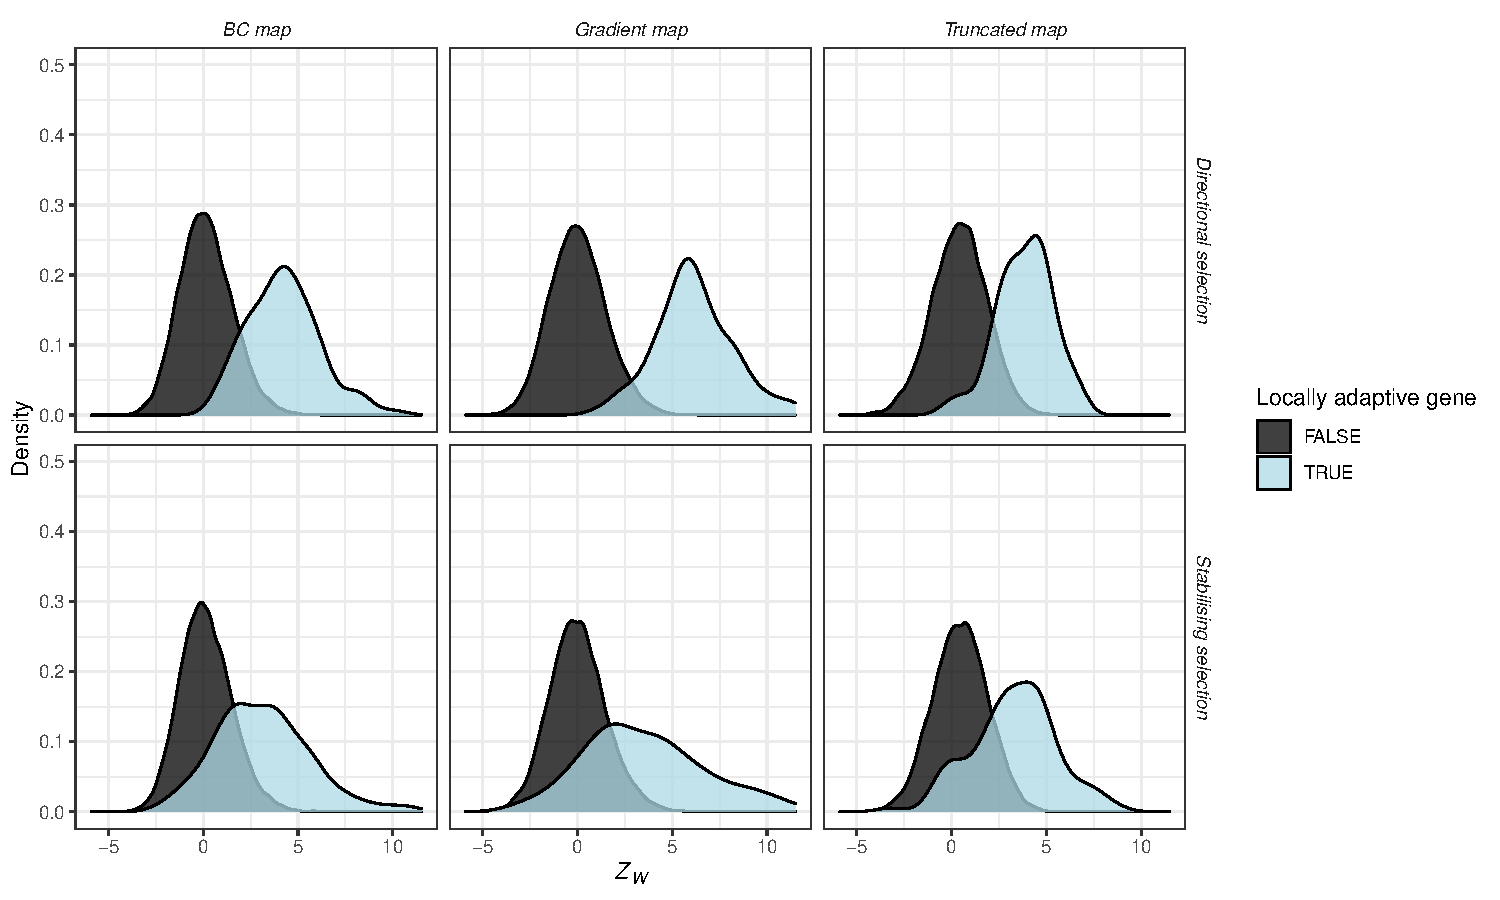
\includegraphics[width=\textwidth,height=0.75\textheight,keepaspectratio]{Plots/selectionWZA_plot.pdf}
  \caption{The distribution of WZA scores from simulations of local adaptation. Note, the plot does not indicate the relative frequency of genes that are or are not locally adaptive. }

  \label{fig:ZScoreDistribution}
\end{figure}

\pagebreak


\begin{figure}[H]
  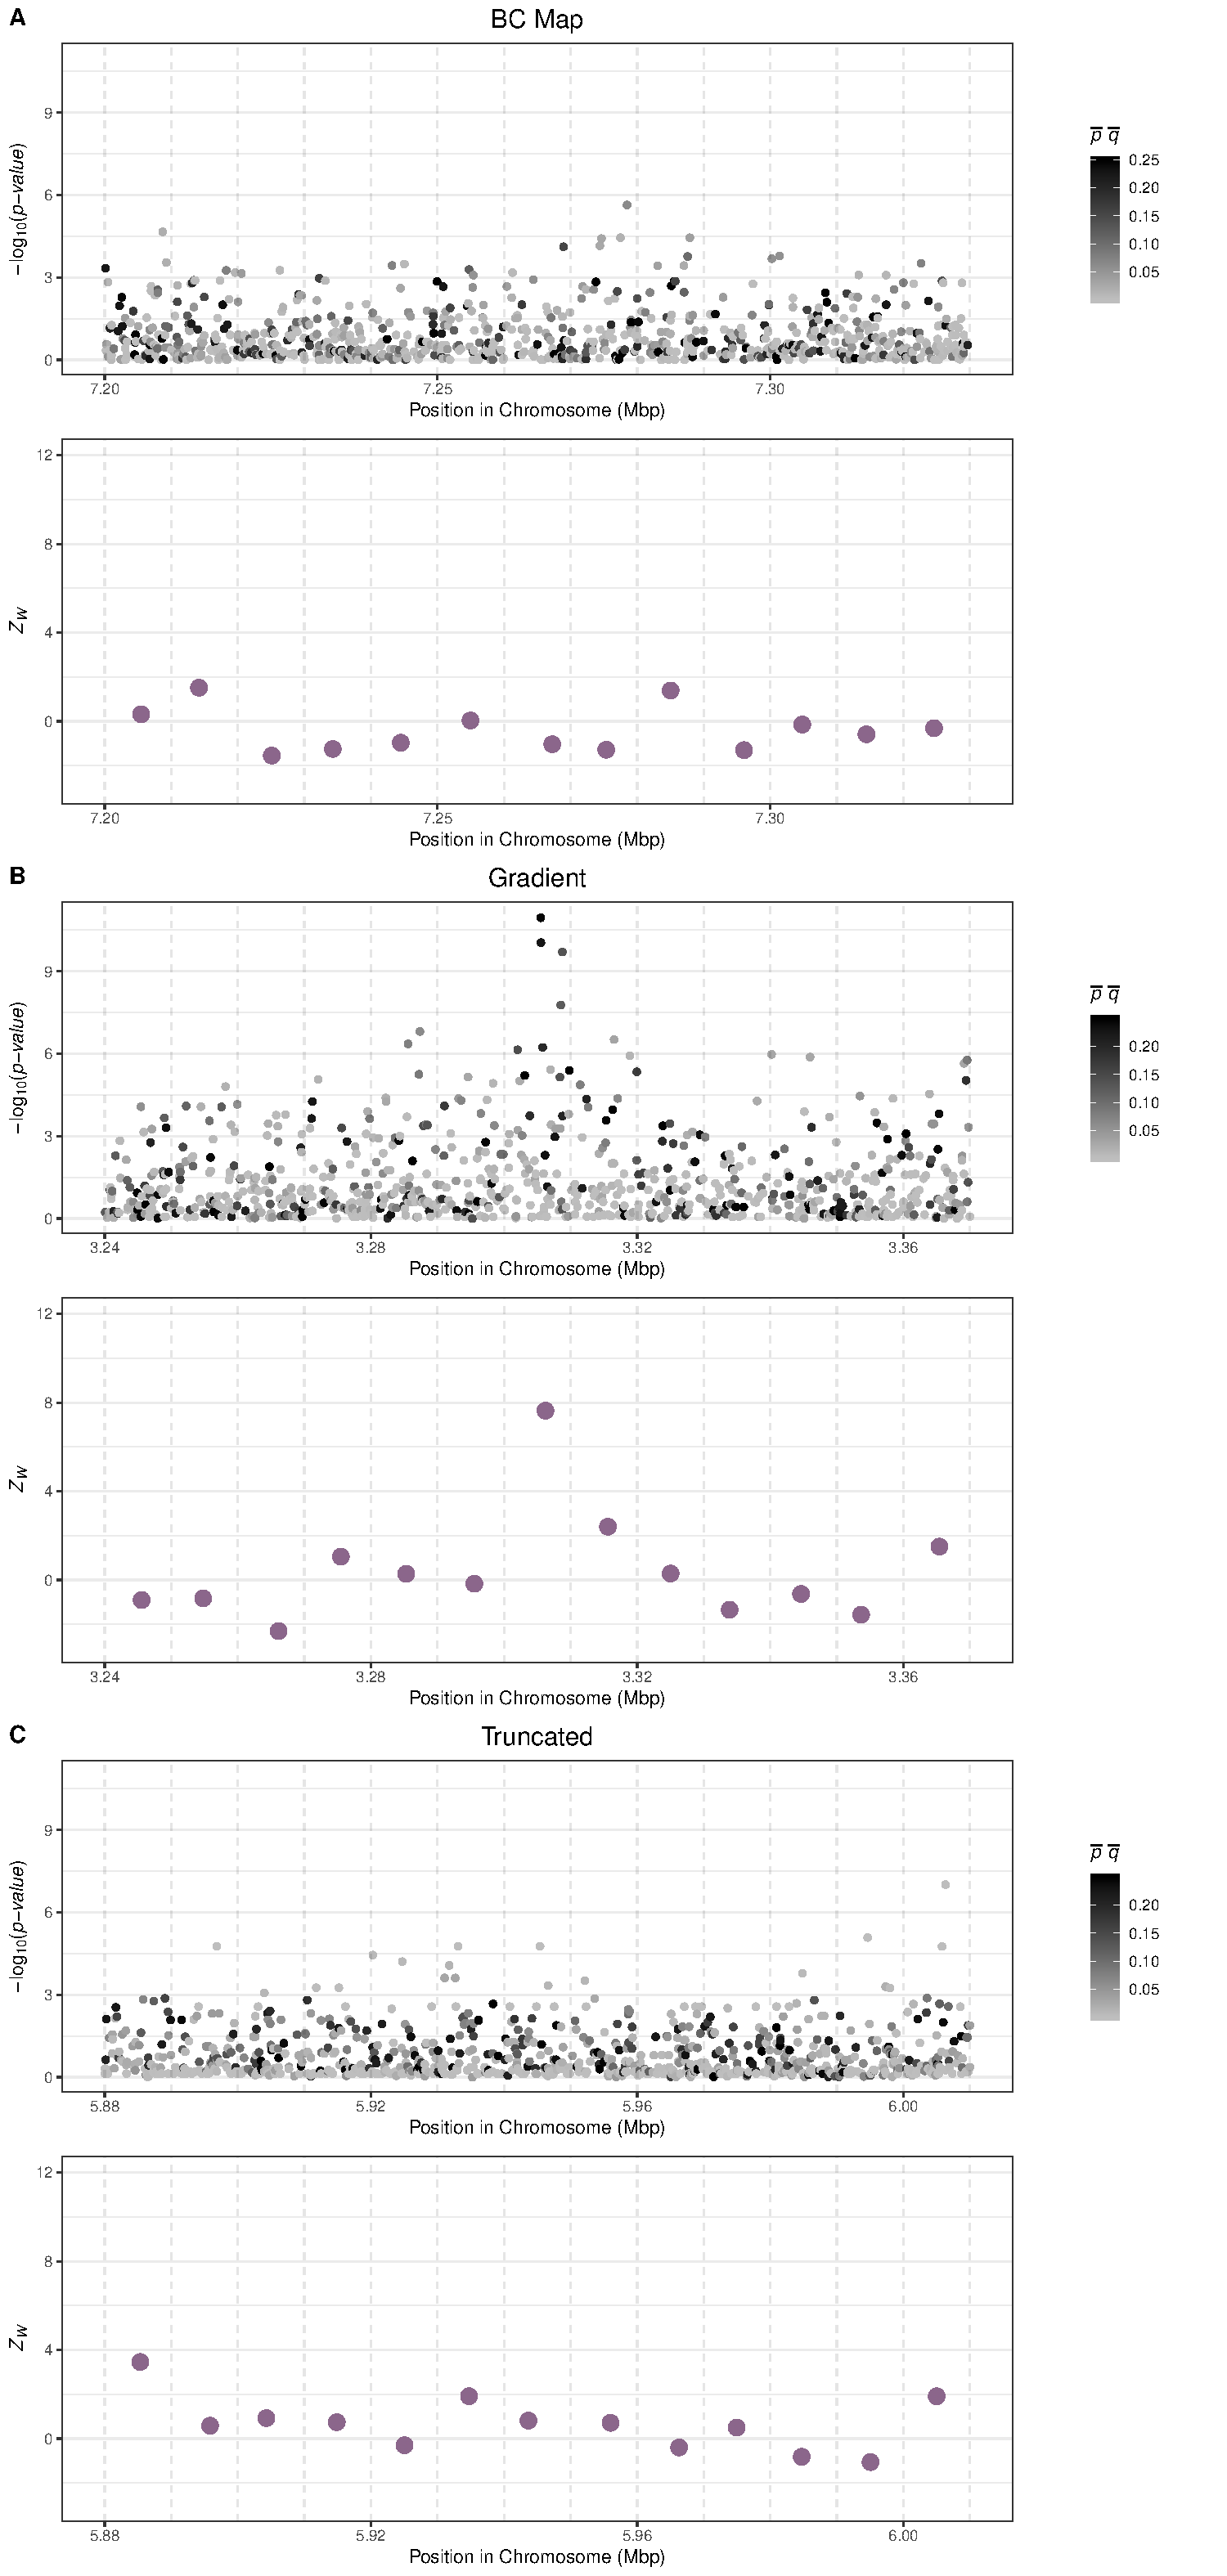
\includegraphics[height=0.9\textheight,keepaspectratio]{Plots/all_maps_plot_demo.pdf}
  \caption{Plots demonstrating the genomic landscape of genotype-environment correlations around a true positive (i.e. a gene that contributes to local adaptation) for the three maps of environmental heterogeneity we simulated. In each panel, the upper plot shows the \textit{p}-value of Kendall's $\tau$ correlation between population allele frequencies and the environment, the lower plot shows the $Z_W$ score for each gene. The boundaries of genes are indicated by the dashed grey vertical lines. Note that the boundaries of genes recombined at a rate that was 50$\times$ higher than the background rate. }

  \label{fig:demoPlots}
\end{figure}

\pagebreak

\begin{figure}[H]
  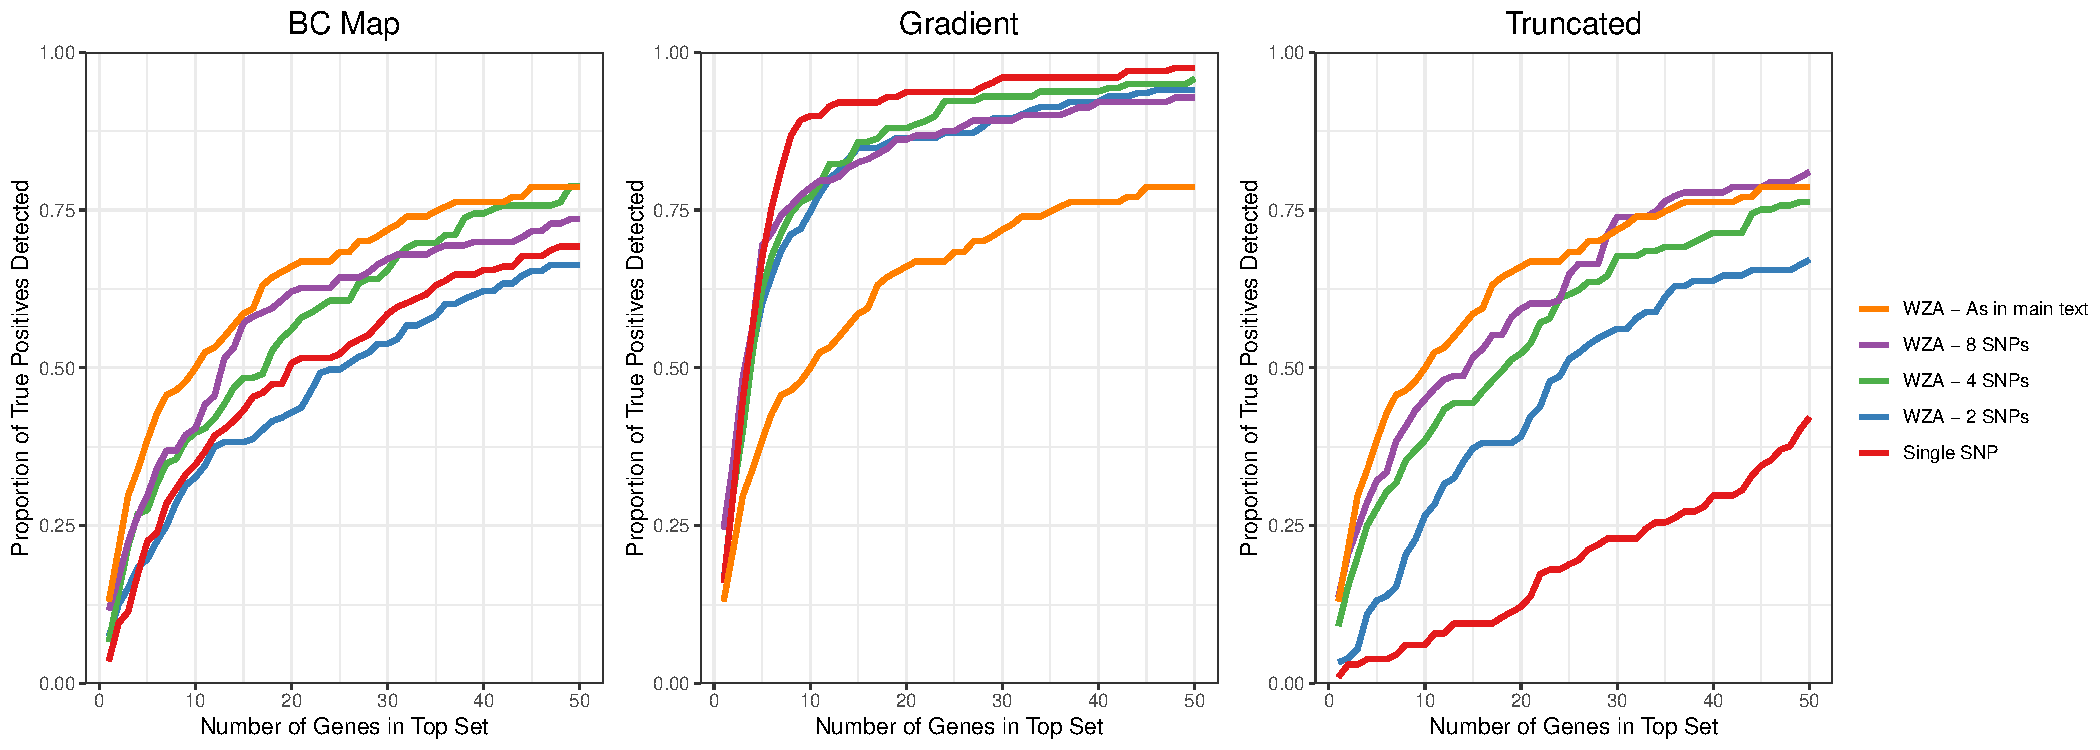
\includegraphics[width = \textwidth,keepaspectratio]{Plots/SNP_number.pdf}
  \caption{Comparing the performance of the WZA genes identified using the WZA, using analysis windows analysing a fixed number of SNPs.}

  \label{fig:demoPlots}
\end{figure}

\pagebreak


\begin{figure}[H]
  \includegraphics[width = \textwidth,keepaspectratio]{Plots/SampleSizeComparison.pdf}
  \caption{Comparison of the WZA, the top-candidate and the single-SNP approaches with varying numbers of sampled demes. Simulations shown assumed the \textit{BC} map and directional selection. Note that the \textit{n = 40} panel is shown as part of Figure \ref{fig:truePosBoth} in the main text. Lines represent the mean of 20 simulation replicates.}

  \label{fig:sampleSize_demes}
\end{figure}

\pagebreak

\begin{figure}[H]
  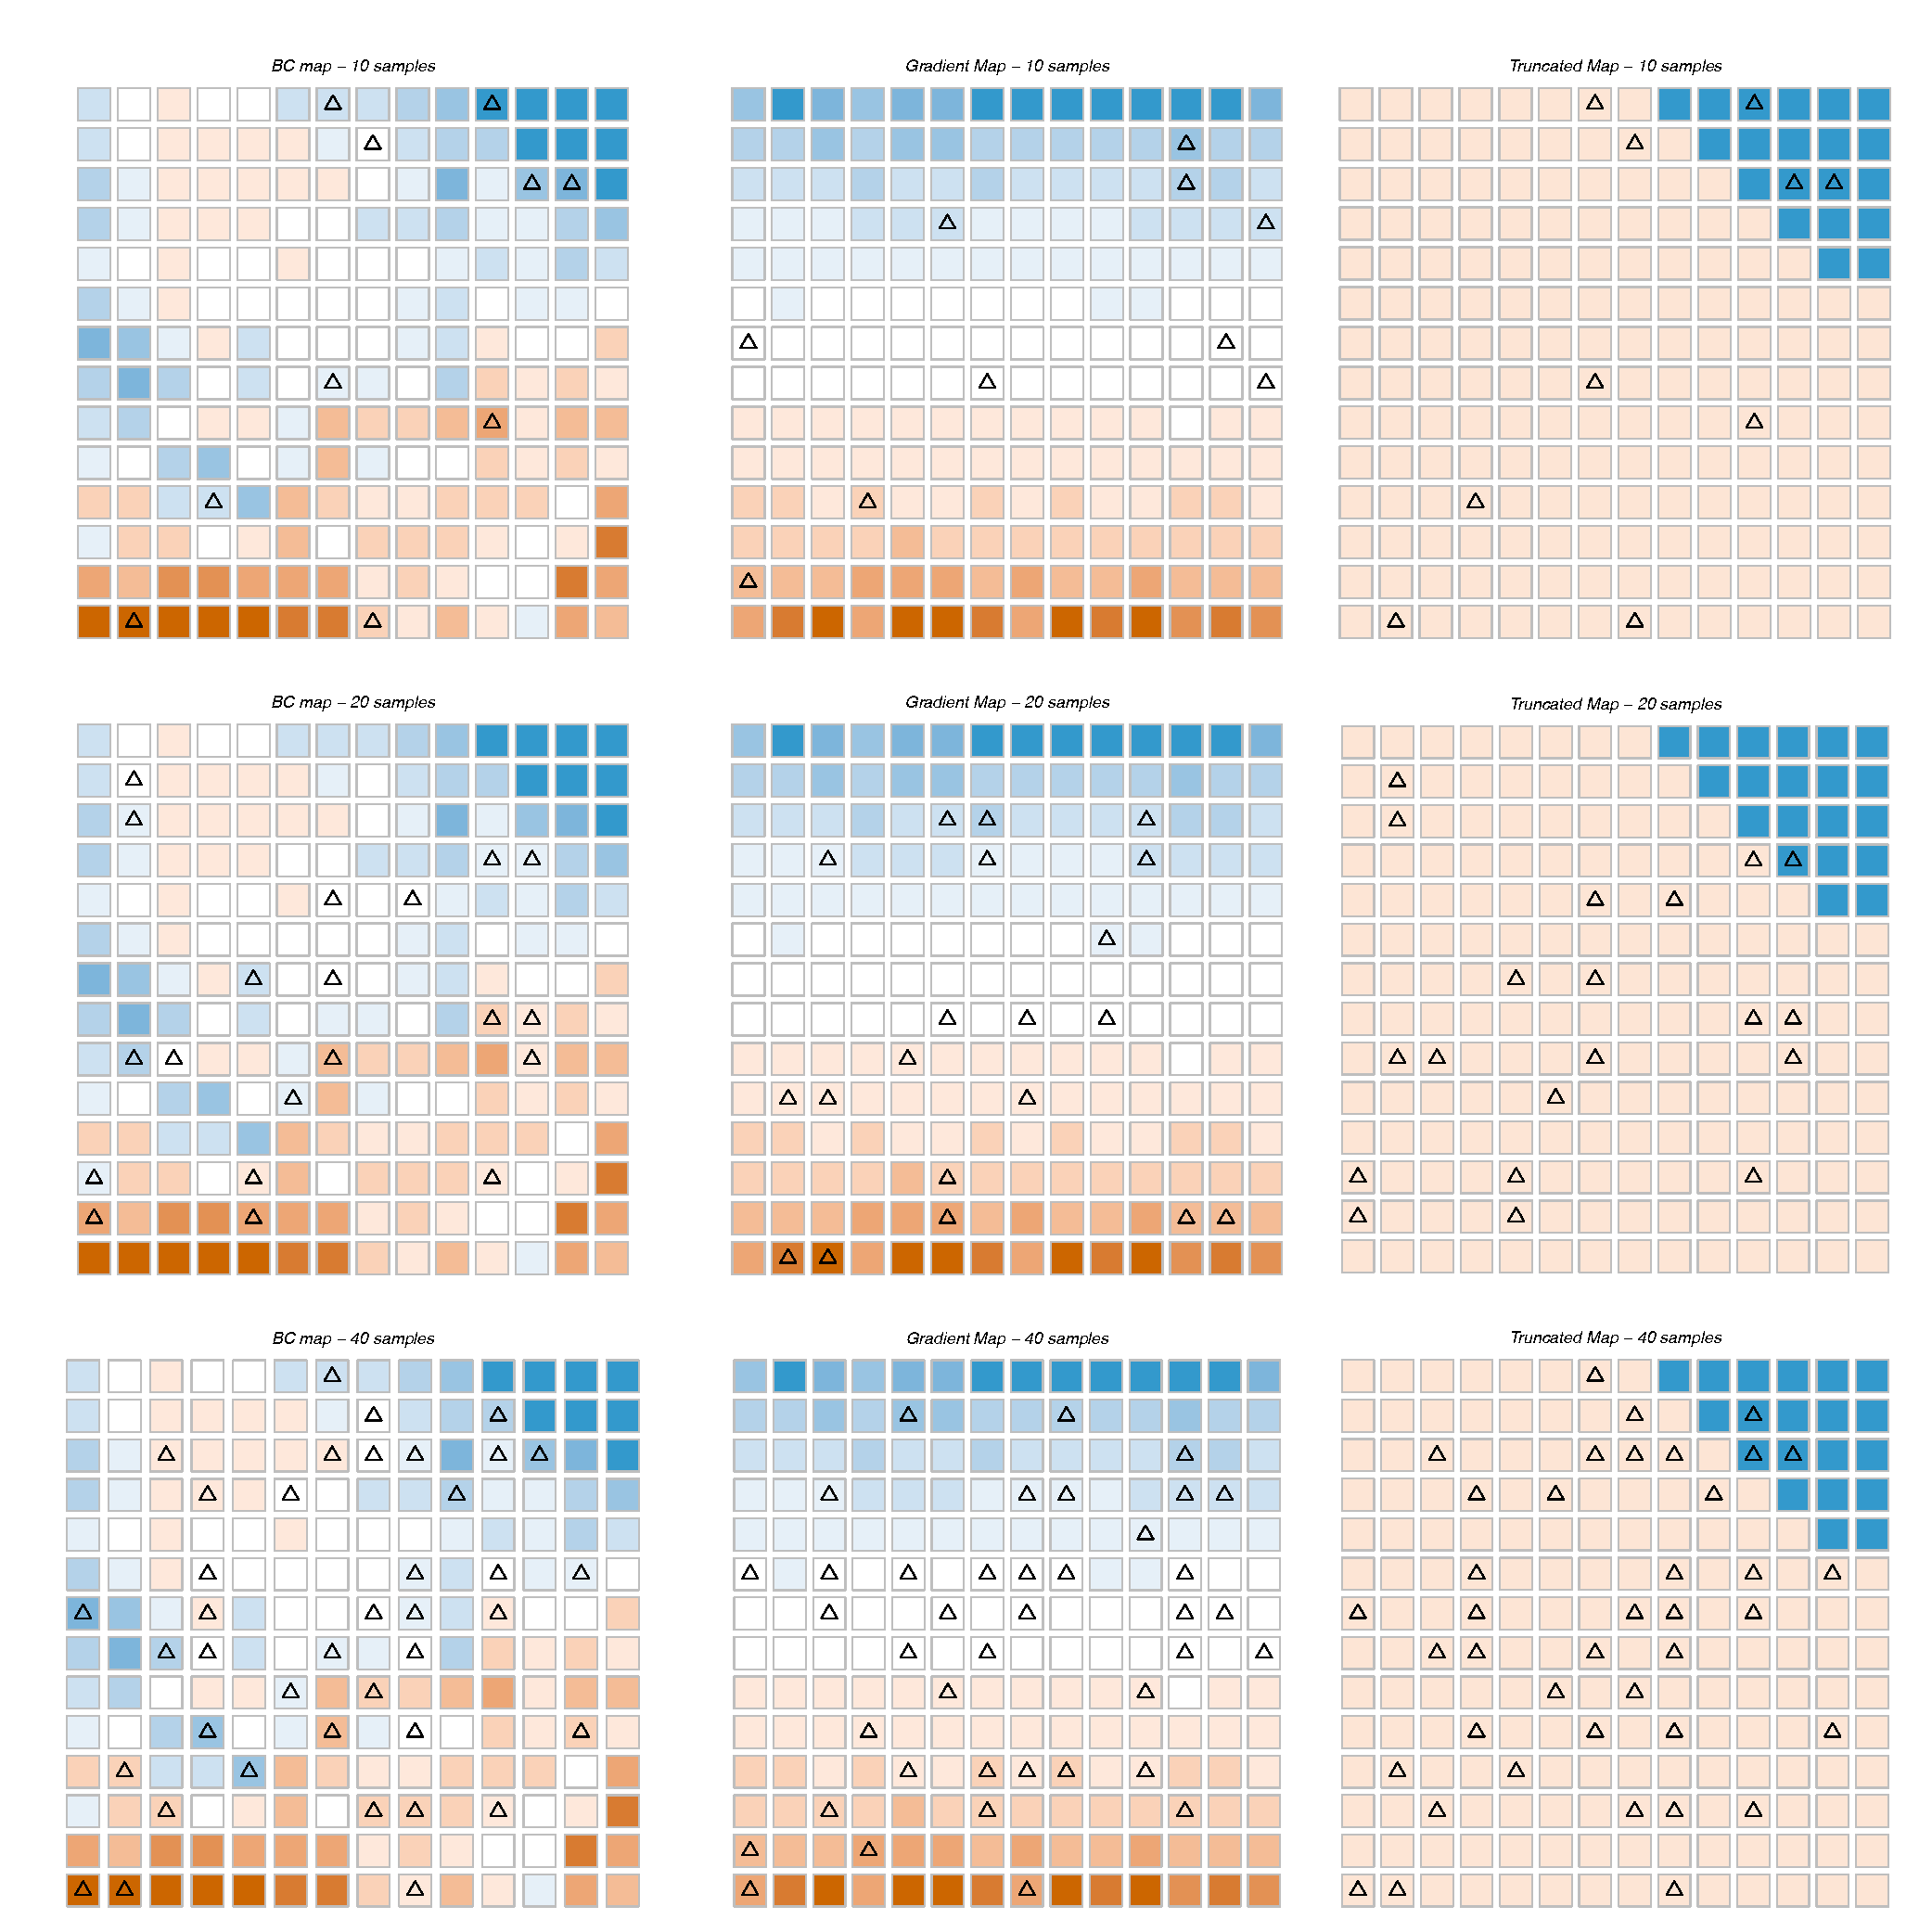
\includegraphics[width = \textwidth,keepaspectratio]{Plots/sample_maps.pdf}
  \caption{Comparison of the WZA, the top-candidate and the single-SNP approaches with varying numbers of sampled demes. Simulations shown assumed the \textit{BC} map and directional selection. Note that the \textit{n = 40} panel is shown as part of Figure \ref{fig:truePosBoth} in the main text. Lines represent the mean of 20 simulation replicates.}

  \label{fig:sampleMaps}
\end{figure}

\pagebreak

\begin{figure}[H]
  \includegraphics[width = \textwidth,keepaspectratio]{Plots/SampleSizeComparison_individuals.pdf}
  \caption{Comparison of the WZA, the top-candidate and the single-SNP approaches with varying numbers of sampled demes. Simulations shown assumed the \textit{BC} map and directional selection. Note that the \textit{n = 40} panel is shown as part of Figure \ref{fig:truePosBoth} in the main text. Lines represent the mean of 20 simulation replicates.}

  \label{fig:sampleSize_individuals}
\end{figure}

\pagebreak
\begin{figure}[H]
  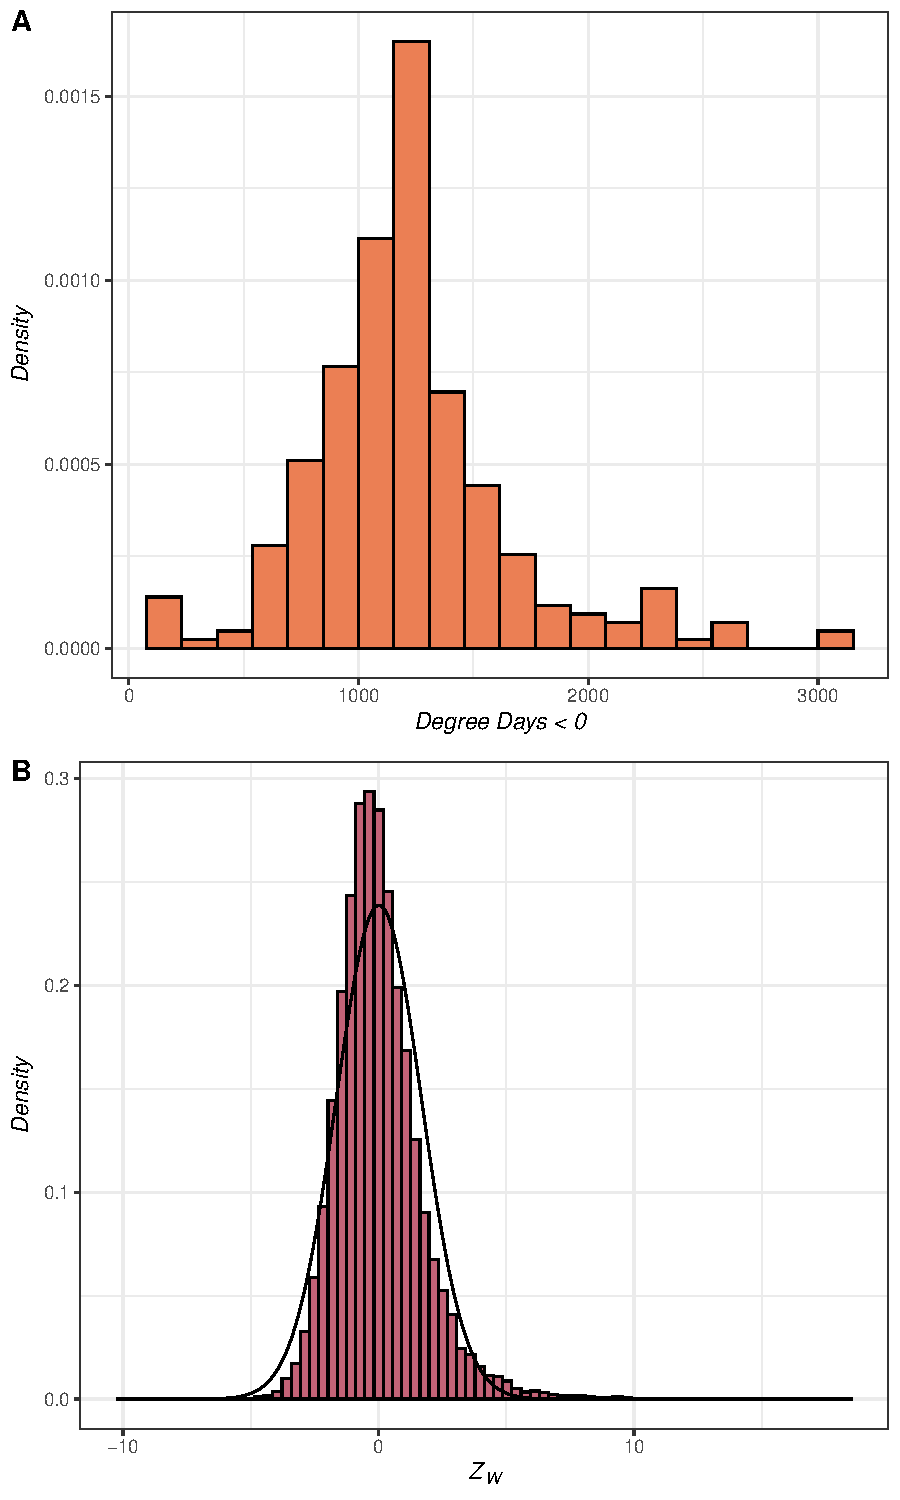
\includegraphics[width=0.75\textwidth,height=0.75\textheight,keepaspectratio]{../dataAnalsis/pineAnalysis_SuppFig.pdf}
  \caption{The distribution of A) degree days < 0 (DD0) across the populations of \textit{P. contorta} sampled by Yeaman et al (2016) and B) $Z_W$ scores for the GEA on DD0. Note that the DD0 values in A) are unscaled. In B) the curve shows a normal distribution fitted to the data.}

  \label{fig:lodgepoleDescriptives}
\end{figure}



\begin{figure}
  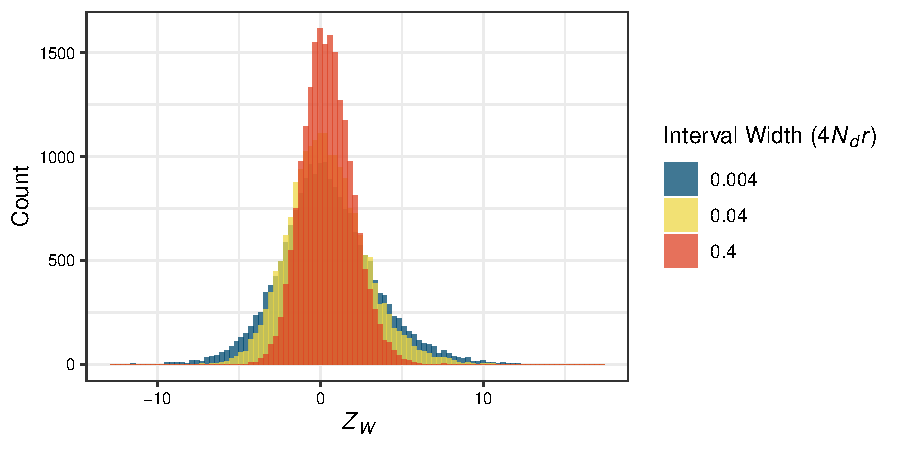
\includegraphics[width=\textwidth]{Plots/recombinationRateHistogram.pdf} 
  \caption{The distribution of $Z_W$ scores under different recombination rates.}
  \label{fig:WZA_Recombination}
\end{figure}


\end{document}





\subsection{Recombination rate variation}

